\chapter{Using Bad Learners to find Good Configurations}
\label{chapter:rank}

To solve the CAT problem,
one-shot prediction (such as \paris~\cite{Yadwadkar2017}) suffers from
high variance of prediction error
while \bo (such as \cherrypick~\cite{Alipourfard2017} and \arrow~\cite{Hsu2018Arrow},
described in Chapter~\ref{chapter:arrow}) must
tolerate the \emph{cold-start} issue.
In this chapter, we design and implement an
effective, efficient and reliable system that recommends
the best architectural configurations 
that satisfies performance and cost objectives
to run a given workload.


\section{Introduction}
\label{sec:introduction}


This chapter presents \scout, which 
identifies search regions that contain suitable architecture configurations.
\scout follows sequential model-based optimization (SMBO)
that converges to the best architectural configurations.
This method better tolerates high variance of the prediction error
in a machine learning based prediction model.
Second, \scout adopts pairwise comparison for determining
the next architectural configurations
that are likely to improve upon the current choice.
Instead of predicting workload performance directly
(\eg in \emph{CherryPick} and \emph{PARIS}),
\scout uses relaxed modeling to find
the next \emph{better} choices (relative ordering).
This naturally fits into SMBO.
Third, \scout uses low-level performance metrics
to identify performance bottlenecks and
to capture cost-performance relationship.
Last, \scout uses transfer learning to acquire knowledge of CAT
from other workloads.
These four elements enable \scout to navigate through the search space
more quickly and intelligently.

Any search-based method has two aspects.
\vspace{-0.5em}
\begin{itemize}
    \setlength\itemsep{-0.4em}
    \item \textit{Exploration:} Gather more information about the search space by executing a new cloud configuration.
    \item \textit{Exploitation:} Choose the most promising configuration based on information collected.
\end{itemize}
\vspace{-0.5em}
Additional exploration incurs higher search cost and insufficient exploration may lead to sub-optimal solutions.
This is the exploration-exploitation dilemma the appears in many machine learning problems~\cite{kaelbling1996reinforcement}.
For example, \emph{CherryPick} requires a good exploration strategy
to characterize the search space~\cite{Alipourfard2017}.

In this chapter, we demonstrate that it is possible to
trade exploration for exploitation
without settling for a sub-optimal configuration.
The central insight of this work is that the cost of the search
for the right cloud configuration can be significantly reduced
by using information gathered during tuning.
However, prior work such as \emph{CherryPick} and \emph{Arrow}
learns from an optimization process of a single workload
~\cite{Alipourfard2017, Hsu2018Arrow}.
This produces unnecessary search cost on exploration
(related to the \emph{cold-start} problem) and
may eventually lead to sub-optimal choices (due to irregular search space).
\scout is able to alleviate these problems
with \emph{transfer learning}~\cite{pan2010survey}---
the knowledge is transferred from previous (but distinct) workloads
using relative ordering and low-level performance metrics,
which does not require workload information.

In this chapter, we identify the key components for an effective method
to the CAT problem.
\scout enables practitioners to find a near-optimal
cloud architecture configuration
with a better search performance and a lower search cost than
the state of the art.
Our key contributions are:

\begin{enumerate}[leftmargin=*]
\setlength\itemsep{-0.4em}
\item we propose a novel system, \scout, that
finds (near) optimal solutions and solves the shortcomings of prior work.
(Section~\ref{sec:approach});
\item we present a novel way to represent the search space,
which can then be used to transfer knowledge
from historical measurements(Section~\ref{sec:approach});
\item we compare the performance of \scout with
other state-of-the-art methods
using 125 workloads and 87 architecture configurations
on three different data processing systems.
(Section~\ref{sec:evaluation}); 
and
\end{enumerate}
%\section{Why Collective Optimization}
\label{sec:motivation}

A cloud optimizer is often evaluated with search performance and measurement cost.

\begin{itemize}
\item \textbf{Search performance} is the measure of the quality of the found solutions by an optimizer.
For example, in searching for the most cost-effective configuration, an optimizer that finds a configuration that is only 10\% more expensive than the optimal is considered better than another optimizer
that can only find a configuration that yields 30\% more cost.
Therefore, we use normalized performance (to the optimal) for evaluation.

\item \textbf{Search cost}
is the total cost of running an optimizer.
An optimization process is expensive because it requires
to test a workload on some cloud configurations for deriving
the best choice.
We use the number of tests as the search cost (or measurement cost)
because it is an intuitive measure.
The amount of charge is another measure~\cite{Alipourfard2017}. 

\end{itemize}


There is always a trade-off between measurement cost and search performance.
The primary motivation for collective optimization is to reduce high measurement cost of optimizing multiple workloads.
If users demand strict search performance, they better turn to single-optimizers.
However, we argue that collective optimization is promising
because it achieves comparable or slightly worse search performance
while reducing measurement cost significantly.
In the following,
we discuss the benefits of having a collective optimizer.


\begin{itemize}
\item \textbf{Large scale cloud migration.}
Cloud computing is a cost-effective solution.
Enterprises are moving in-house applications to the cloud,
and need a quick way for large migration~\cite{khajeh2010cloud,sripanidkulchai2010clouds}.
Elaborate optimizers are expensive (in measurement cost) and time-consuming (in optimization process).

\item \textbf{Limited budgets.}
The single-optimizer such as \emph{CherryPick} and \emph{Scout} are effective and desirable for highly recurring workloads because the measurement cost can be amortized.
However, the number of budgets to run optimizers
does not increase linearly with the number of workloads.
To better support multiple workloads,
we need to reduce measurement cost while delivering comparable search performance.

\item \textbf{Expanding cloud portfolio.}
Cloud providers expand their cloud portfolio more than 20 times in a year~\cite{ec2history}.
Therefore, users have to rerun optimizers to update their configurations for all workloads.
Again, this is an expensive and time-consuming process.

\item \textbf{Seed cloud optimizers.}
All the cloud optimizers require initial measurements.
It is unclear how to determine the best starting points.
We aim to find the exemplar configurations,
which can be used as the starting points, thereby
reducing measurement cost.
The exemplar configuration can be used to seed singe-optimizers such as CherryPick and \scout, which will be discussed more in Section~\ref{sec:system}.

\end{itemize}

In summary, users would prefer collective optimization if search performance is comparable to single-optimizers while measurement cost can be reduced greatly.

\section{Design Choices}
\label{sec:design}

\begin{figure}
\resizebox{.8\linewidth}{!}{%
    \small{
        \begin{tabular}{@{}lccccc@{}}
        \toprule
        \textbf{Methods} & \textbf{\begin{tabular}[c]{@{}c@{}}Search-\\ based\end{tabular}} & \textbf{\begin{tabular}[c]{@{}c@{}}Relative\\ Ordering\end{tabular}}  & \textbf{\begin{tabular}[c]{@{}c@{}}Low-level\\ Metrics\end{tabular}} & \textbf{\begin{tabular}[c]{@{}c@{}}Historical\\ Data\end{tabular}} & \textbf{\begin{tabular}[c]{@{}c@{}}Transfer\\ Learning\end{tabular}} \\ \midrule
        CherryPick~\cite{Alipourfard2017} & \cmark & \xmark & \xmark & \xmark & \xmark \\
        PARIS~\cite{Yadwadkar2017} & \xmark & \xmark & \cmark & \cmark & \xmark \\
        Arrow~\cite{Hsu2018Arrow} & \cmark & \xmark & \cmark & \xmark & \xmark \\
        \cellcolor[HTML]{9B9B9B}\textcolor{white}{\textbf{Scout}} & \cellcolor[HTML]{9B9B9B}\color{white}\cmark & \cellcolor[HTML]{9B9B9B}\color{white}\cmark & \cellcolor[HTML]{9B9B9B}\color{white}\cmark & \cellcolor[HTML]{9B9B9B}\color{white}\cmark & \cellcolor[HTML]{9B9B9B}\color{white}\cmark \\ %\bottomrule
        \end{tabular}
    }
    }
    \centering
    \caption{
    \small{
    \textbf{An overall comparison with other CAT methods.}
    A search-based method better tolerates prediction bias.
    Relative ordering better captures the workload-architecture-performance relationship.
    Leveraging low-level metrics improves search performance.
    Historical data helps eliminate unnecessary exploration overhead in a search.
    Transfer learning greatly reduces search cost.}
    }
    \label{fig:model_classification}
\end{figure}


By analyzing the differences between the state of the art methods,
we identified the following key components in solving the CAT problem:
(1) a search-based method (similar to \emph{Cherrypick}~\cite{Alipourfard2017})
is essential since it accommodates mispredictions and performance variances
in the cloud,
(2) relative ordering better captures
the workload-architecture-performance relationship,
which creates fewer mispredictions,
(3) low-level performance metrics are a good proxy of
predicting system performance~\cite{Novakovic2013,Hsu2016,Yadwadkar2017},
(4) historical data (as used in PARIS~\cite{Yadwadkar2017}) is useful
to understand the inherent preferences of a workload, and
(5) transfer learning boosts search performance and improves convergence speed
by minimizing exploration phase.
These components together solve the CAT problem more effectively
and overcome the shortcomings of the current state of the art approaches.
\myfigure{\ref{fig:model_classification}} compares and contrasts the
design choices of \scout against prior work.

Because it is a daunting task to build an accurate model that
predicts performance and cost of workloads on
distinct cloud architectural configurations,
we can instead build an indirect model (for improving prediction accuracy).
A search-based method does not require a direct answer
(which choice is the best),
but an answer to ``are there better choices?''
We do not predict the absolute performance of a configuration but rather
predict the relative performance of two configurations.
That is, we can simplify the prediction model that will assist
a search-based method in finding the solutions more efficiently~\cite{nair2017}.
\emph{Learning to rank} is an important machine learning task
~\cite{harrell2001ordinal,li2008mcrank,cao2007learning}.
We prefer relative ordering instead of total ordering for
ranking architectural configurations because
there does not exist a one-size-fits-all architecture
for any workloads and for any objectives.

SMBO requires exploration efforts
(increases search cost)
to update its belief (prediction) on the search space.
However, the data for the initial model need not come from
the workload being evaluated.
Rather, data from any workload can be used to build a useful model describing
the search space.
For this model to be most useful, the information must be generic---independent
of workloads.
This technique is inspired by \cite{Hsu2016,Yadwadkar2017}.
There are too few features (dimensions and options) in the configuration space
to build a robust model that works across many workloads.
Consequently, a model based only on architectural features
(\eg{cluster sizes and memory per core}) is fragile.

To summarize, the following elements are necessary
to create an effective approach.
\begin{enumerate}[leftmargin=*]
    \setlength\itemsep{-0.4em}
    \item Prefer the \textbf{\textit{search-based technique}}, which converges to the best solution iteratively and avoids the large penalty caused by dramatic prediction error.
    \item Use a \textbf{\textit{relaxed}} model that boosts prediction accuracy, thereby better guides a search process to find the near-optimal configurations more quickly,
    \item Use \textbf{\textit{low-level metrics}} to generate a generic representation of the search space such that it can be used by other combinations of workload and application.
    \item Create a \textbf{\textit{performance database}} so that the knowledge of optimization can be used by other optimizers to find the right cloud configuration and hence reduce the search cost. 
\end{enumerate}
\section{From Observation to Action}
\label{sec:approach}
In this section, we describe how to derive search hints from performance data
to guide a search process.

\subsection{Exploration vs. Exploitation}

A search-based method navigates in the search space
to find the best cloud architectural configuration.
It is mostly concerned with
two questions:
``what are better choices?'' and
``what are more promising regions?''
The former ensures that a search will
eventually, find a near-optimal configuration
while
the latter determines how quickly it finds the solution
(also known as convergence speed).
An effective and efficient search method must answer
these two questions.

To this end, we actually need only to know ``what are better choices?''
At each step, a search-based method aims to find a cloud configuration
that is better than the current best.
A higher probability of \emph{guessing} the next step right
ensures that a search process sequentially finds a better choice.
A right next step also guides a search process
to move towards the right direction.
As long as the optimizer can move closer to the desired solution at each step,
it is more likely to guarantee it will find
near-optimal solutions.

To better determine the next step, a search process can learn
from the observations along the search path.
However, this method faces two challenges.
First, it requires collecting sufficient data to build strong belief.
\emph{CherryPick} is confronted by the cold-start issue
since it must first explore the search space---to identify the promising regions.
Second, an insufficient number of observations leads to
high bias in prediction---the method can wrongly believe that
a particular region (such as VM types or cluster sizes) is more promising
than the other, leading to a sub-optimal solution.

Instead of learning only from observations collected
while executing the target workload, a search process also can learn from
performance data of other workloads---which have been optimized in the past.
This addresses the issue of high bias because a larger number of
measurements (performance data) is available to create a prediction model that
generalizes a performance model better.
This also sidesteps the exploration problem because the search process
does not need to collect observations by running workloads
of the current search task.
The idea of reusing the data is often tricky
since the different combination of application and workload exhibit
very different behavior.
For example, the same application with different inputs can create
very different workload behavior
(such as the execution time and running cost)~\cite{Hsu2018Arrow}.
A performance model, which captures this complex behavior requires
more information about the search space than just
the architecture level information such as VM types and cluster sizes.


\subsection{Core Techniques}
To navigate the search space efficiently, \scout is built on
the following four ideas.


\subsubsection*{Pairwise comparison}
A search-based method determines the next configuration to evaluate.
That is, the method only needs to rank
the set of unevaluated cloud configurations.
Therefore, we can use \textit{Pairwise Comparison} modeling scheme~\cite{wauthier2013efficient}.
\emph{CherryPick} uses Gaussian process to build prediction model,
$f(x_i, K) = y_i$, where $x_i$ is the feature vector to represent
an architecture configuration and $K$ is the covariance kernel function.
With pairwise comparison, the learning task is
\begin{equation} \label{eq:1}
f(x_i, y_i, x_j) = y_j,
\end{equation}
where $x_i \in E$ and $x_j \in S-E$.
In words, it predicts the cost ($y_j$) of a configuration not yet
evaluated ($x_j$) given the cost ($y_i$) from the best configuration
yet found ($x_i$).
This modeling technique does not require to make an assumption ($K$) about
the search space (which is another hyper-parameter to tune),
and
naturally fits into SMBO in updating belief upon new observations.
For the same workload, switching
from a smaller VM type (\eg{\emph{large}}) to a larger one (\eg{\emph{2xlarge}})
may result in different performance on different VM families
(\eg{\emph{c4} and \emph{r4}}).
This performance relationship may change dramatically due to workload changes.
Regression-based modeling needs to fit the corresponding features accurately
for predicting performance~\cite{rasmussen2004gaussian,wettschereck1997review}.
Pairwise comparison helps capture performance transition
between architectural configurations.
Although there are $P(n,2)$ pairs (permutation),
where $n$ is the number of configurations,
in practice, we do not have to obtain full pairs for training this model.
This is because some pairs, \eg{(\emph{c4.large}, \emph{r4.large})}, show
significant performance differences in comparison with other pairs,
\eg{(\emph{m4.large}, \emph{r4.large})}.

\subsubsection*{Relative ordering}
Ranking architectural configurations does not need to predict
absolute performance (a harder problem).
Besides, ``a bad learner'' sometimes can still find a good solution~\cite{nair2017}. 
The idea of using an inaccurate model is useful
because the effort required to build an accurate model is much higher than
an inaccurate model.
%Hence, we do not need to predict performance directly rather
%the relative ordering or ranks.
%\ick[redundant with above?]
Based on this insight, we choose not to infer (inaccurate) performance measure
but rather to infer (accurate) relative ordering---
one configuration is better than another.
To support relative ordering, we modify the learning task from
\myequation{\ref{eq:1}} to
\begin{equation} \label{eq:2}
f(x_i, x_j) = \sigma({\frac{y_j}{y_i}})
\end{equation}
where $\sigma$ is a ranking function.
Binary ranking (\ie{better or worse}), for example, is the simplest form.
This transformation simplifies the learning task because
it does not predict absolute performance.
Furthermore, a coarse-grain ranking function better tolerates
performance variance in the cloud because
a small variance may still result in the same ranks.
%This technique trades search cost for search performance.
\myfigure{\ref{fig:reg_clas}} shows that the prediction accuracy of
relative ordering (using classification) is higher than
total ordering (using regression).
This experiment uses \emph{ExtraTrees}~\cite{geurts2006extremely} in
both the regression and classification task for fair comparison.
The increase in prediction accuracy greatly reduces search cost because
it is more likely to avoid wrong predictions (see Section~\ref{sec:why_better}).


\subsubsection*{Low-Level Insight}
Low-level performance metrics help identify
performance problems~\cite{Bodik2010, Novakovic2013} and
predict application and system performance~\cite{Hsu2016,Yadwadkar2017}.
Understanding resource bottlenecks helps choose the right cloud configuration and helps \scout ignore not so promising cloud configurations.
For example, in optimizing execution time, a memory bottleneck indicates
an instance with larger memory may improve resource efficiency,
thereby reducing execution time.
With low-level performance information, our learning task becomes
\begin{equation} \label{eq:3}
f(x_i, m_i, x_j) = \sigma({\frac{y_j}{y_i}})
\end{equation}
where $m_i$ represents the low-level performance vector.
This is similar to the process of
troubleshooting performance problems and
identifying resource bottleneck.
Instead of constructing rules manually,
this learning task can extract those rules implicitly.
When a workload runs inefficiently on one architectural configuration,
\scout observes abnormal or insufficient resource usage.
This observation is translated to prediction probability implicitly.
\scout ignores those configurations with low prediction probability.


\subsubsection*{Transfer learning}
The accuracy of a performance model depends on the number of data points
used to train the model.
In CAT, the data points are expensive to compute.
When building the performance models, it might be best to reference observations
from other optimization processes.
Researchers in transfer learning report that data
from other optimization processes can yield better models
than just using current data~\cite{pan2010survey,peters2015lace2}.
In this work, workloads share the same search space $S$ and therefore,
architectural features are the same.
Besides, \scout uses generic low-level metrics.
These enable transfer learning possible in \scout.
Although including workload information might improve search performance,
it prevents \scout from transferring knowledge
from historical optimization data.

\begin{figure}[t]
 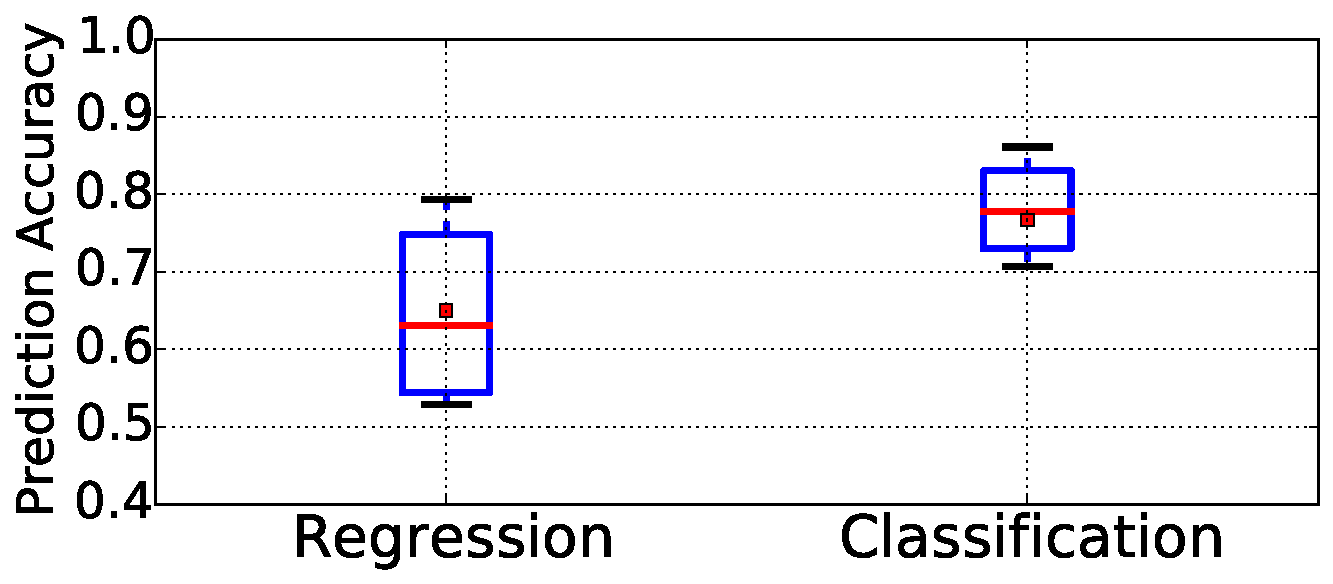
\includegraphics[width=.8\textwidth]{figures/multiple_prediction_accuracy.pdf}
 \centering
 \caption{\textbf{On the model selection of predicting the next step.}
 We evaluate the ability to distinguish a good and a bad configuration.
 In regression, we test rank preserving as prediction accuracy~\cite{nair2017}.}
 \label{fig:reg_clas}
\end{figure}


\subsection{Search Hints}
This section explains how to extract search hints using
probabilistic classification methods
~\cite{friedman2001elements,zadrozny2001obtaining,zadrozny2002transforming}.
A probabilistic classifier predicts probability distribution over
predicted classes.
In \myequation{\ref{eq:3}}, the learning task ranks the relative
performance measure of two architectural configurations.
We can map ranks to classes.
For example, the rank function $\sigma$ outputs \emph{class 1} if
$\frac{y_j}{y_i} < 1.1$. Otherwise, the output is \emph{class 0}.
A binary classifier is able to answer ``is $x_j$ better than $x_i$?''
A probabilistic classifier outputs higher probability for \emph{class 1} if
a specific workload performs better on $x_j$ than $x_i$.

We use an example to illustrate this process.
Consider a configuration space ($S=\{S_1, S_2, S_3, S_4\}$).
An CAT optimizer starts with $S_1$ and $y_1 = \phi(S_1) = 10$ (the current best).
Let us assume we have collected historical data for
training the probabilistic classifier.
The predicted probability distribution over ${S_1, S_2, S_3, S_4}$ 
is $[-, 0.8, 0.2, 0.2]$.
The probability vector $P_{i}$ represents
``how likely $S_j$ is a better choice than $S_i$.''
A higher value indicates $S_j$ is more likely
to perform better than $S_i$. 
In this example, $S_2$ is a better choice than the others.
When the actual performance measure is better $\phi(S_2) \leq \phi(S_1)$,
then CAT optimizer found a better solution than the current best.

The above example uses a binary classifier, and
\scout uses multiclass classification.
The intuition for using multiple classes is that some configurations
yield similar performance, and \scout should not consider little improvement.
For example, we can define the classes to be ``better,'' ``fair,'' and ``worse.''
\scout favors the configurations in the ``better'' class.
\scout uses a predefined discretization policy
(based on user-defined thresholds)  to convert probability to discrete classes.
%For example, $\frac{\phi(S_j)}{\phi(S_i)} \leq 0.8$ is considered as ``better.''
%\ick[do you mean i is better?]


\subsection{Search Strategy}

During the search process, a new observation
(running a workload on a selected cloud configuration)
provides the necessary information to determine
whether there exist better choices (see \myequation{\ref{eq:3}}).
The probability vector $P_{i}$ is derived
for each new observation $\phi(S_{i})$.
A search strategy determines the choice based on the probability predictions.
At each step, the search process selects the configuration $S_j$ with
the maximum probability in $P_{i}$.

This search strategy is similar to depth-first search.
While \emph{CherryPick} requires balancing exploration and exploitation,
\scout tends to exploit---because it uses historical data.
When the prediction model can generate quality predictions,
this search strategy leads to quick convergence speed
(the selected configuration improves over the current best).
Therefore, the search process has low search cost to find near-optimal
configurations. 

A search process should stop when it no longer can find a better configuration. This is controlled by a predefined parameter called  \textit{probability threshold} ($\alpha$) and acts as a stopping criterion.
When the predicted probability $P_{ij}$ is lower than $\alpha$ for all $S_j$,
the search process is not confident that it would find better configurations in the next step.
A search should also stop if it fails to find better solutions due to an inaccurate performance model. This is controlled by another parameter called \textit{ misprediction tolerance} ($\beta$) to avoid excessive search cost.

\subsection{Putting It All Together}
We have shown that the core element of a search based method is to determine
the next best step.
For obtaining hints to guide a search process,
we propose using the probabilistic classification technique
to predict improvement probability.
That is similar to Expected Improvement (EI) in \emph{CherryPick}.
We choose pairwise comparison and relative ordering
to deliver high prediction accuracy and to naturally into the search process.
\scout leverages low-level performance information and
extracts rules (based on resource utilization) implicitly.
This improves a search process because certain types of cloud configurations
can be avoided (as we will show in Section~\ref{sec:evaluation}).
Last, we choose a search strategy that merely picks the configuration
that is most likely to be better than the current best.
This strategy increases convergence speed---has low search cost.

\section{Implementation}
\label{sec:system}

This section describes the implementation of \scout
as shown in \myfigure{\ref{fig:system_design}}.
We implement the system in Python with
scikit-learn~\cite{scikit-learn} for machine learning libraries and
Boto 3~\cite{boto3} for interacting with Amazon web services.


\begin{figure}[!htbp]
 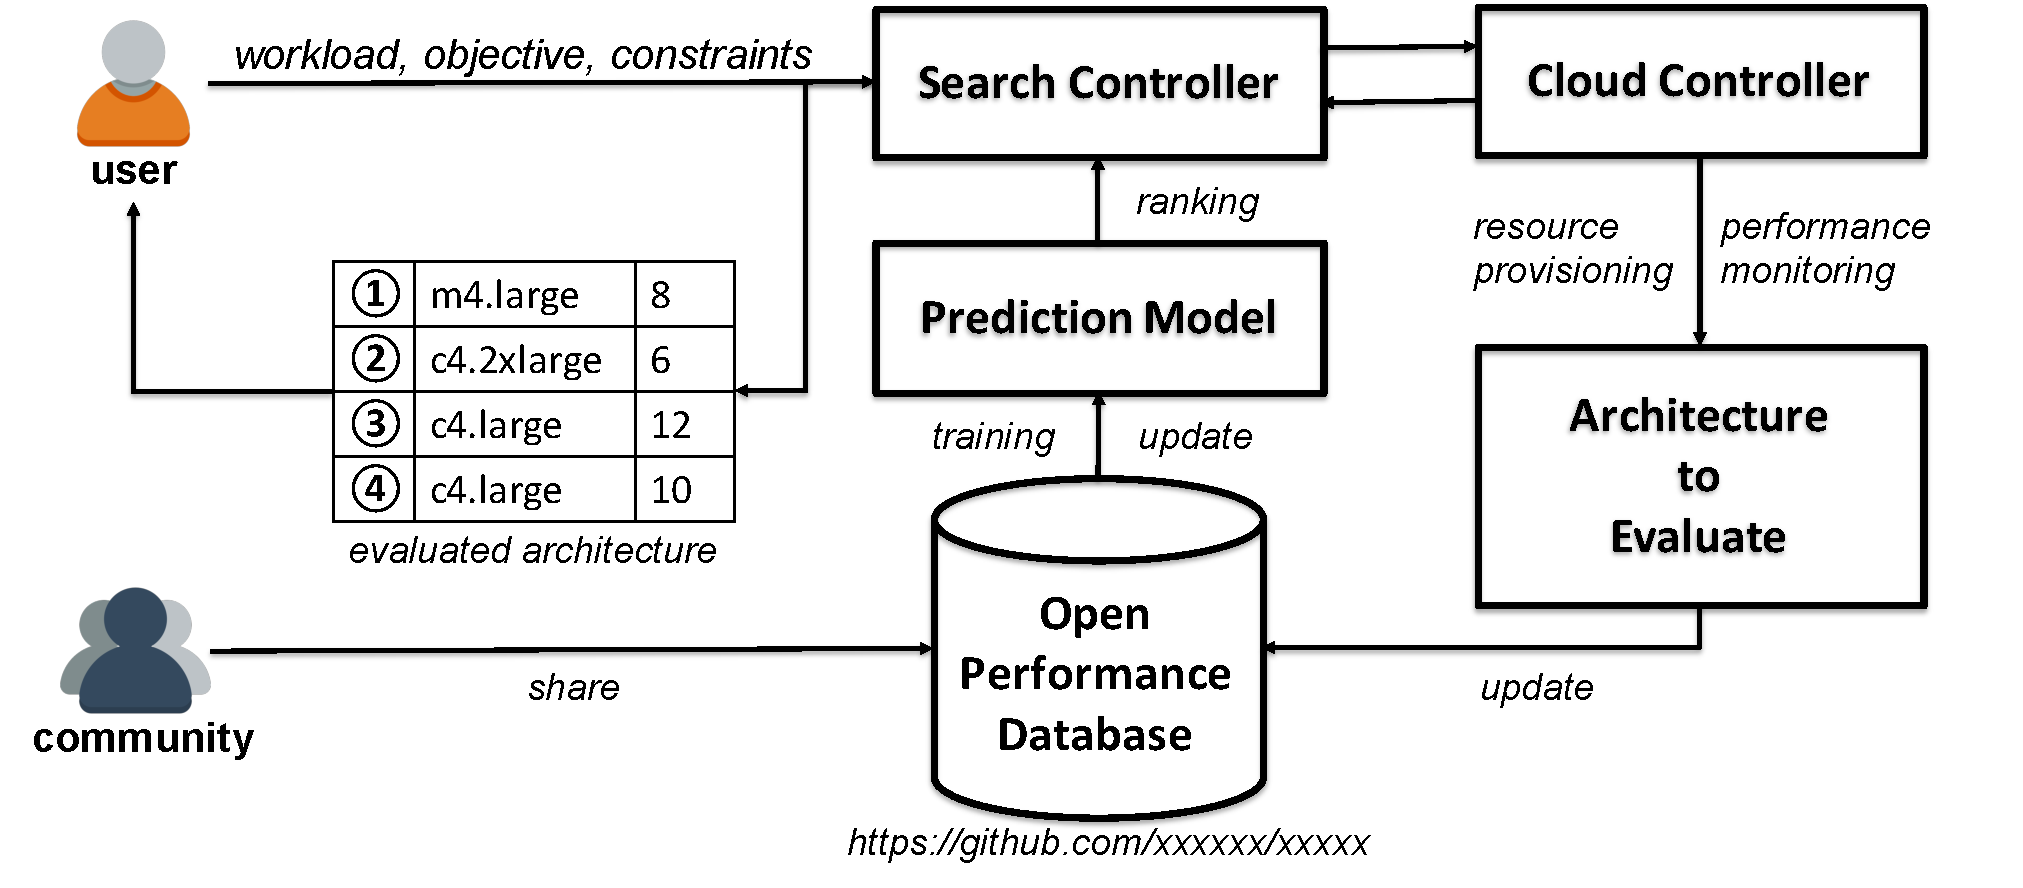
\includegraphics[width=.8\textwidth]{figures/system_design_blind.pdf}
 \centering
 \caption{\small{\textbf{\scout's implementation.}
 }}
 \label{fig:system_design}
\end{figure}


\begin{itemize}
\item \textbf{Search Controller.}
This is the entry point to use \scout.
A user submits a workload along with performance and cost objectives.
The user can also specify constraints such as maximum execution time,
maximum cost budget and the range of cluster sizes, etc.
The performance of \scout is not heavily affected by
the initial architectural configurations.
For evaluations, \scout randomly selects one configuration.
The search controller forwards the workload and the selected configuration
to the cloud controller.
Once the selected configuration is evaluated,
the search controller is notified and determines
the next configuration to evaluate.
\scout selects the configuration that, according to the model, has the
greatest likelihood of improving performance.
% The probability information is provided by the prediction model.
This optimization process stops when the objective is fulfilled or
when the evaluation budget is expended.

\item \textbf{Prediction Model.}
We can use a probabilistic classifier to derive the probability distribution
over prediction classes~\cite{friedman2001elements}.
Possible choices include, but are not limited to,
Logistic Regression, Gaussian Process, Random Forests and neural networks
~\cite{breiman2001random,friedman2001elements}.
\scout uses \emph{ExtraTree}
to train a classification model
for deriving relative ordering (to determine better configurations)
because \emph{ExtraTree} is more efficient and reliable
% to cope -- check this. does it still make your point?
with
numerical performance data~\cite{geurts2006extremely}.

\item \textbf{Cloud Controller.}
The cloud controller bridges the search controller and cloud platforms.
The controller is responsible for running the workload
with a specific architectural configuration.
\scout currently supports AWS but easily can be extended
to other cloud platforms.
For each evaluation, the cloud controller monitors the execution time and
collects low-level performance information.
We use the \emph{Sysstat} package on Linux for system monitoring~\cite{sysstat}.
Since we collect only generic performance metrics, other monitoring tools
should work as well.
We choose a five-second sampling period.
Each sample has 72 metrics from
CPU, memory, cache, disk and network components.
These numbers are then aggregated from various-size
samples (per node) and nodes (per cluster).
We follow the similar process of feature transformation
as described in~\cite{Hsu2016,Hsu2018Arrow}.

\item \textbf{Open Performance Database.}
Performance data is hard to find.
We believe sharing data can greatly advance the research
on CAT.
Moreover, cloud users benefit from the performance database because
they are able to learn the workload performance on
different architecture configurations, which are very expensive
to obtain.

\end{itemize}
\section{Evaluation}
\label{sec:evaluation}

We evaluate \scout with three sets of big data analytics
applications on 18 cloud configurations on a single-node.
We further evaluate 69 cloud configuration on multiple nodes.
Our evaluations show that \scout finds the optimal or near-optimal configuration more often than other methods
and does so while reducing search costs.

\subsection{Experiment Setup}
\label{sec:setup}

\subsubsection*{Workloads}
We choose diverse workloads (CPU-intensive, memory-heavy, IO-intensive and network-intensive) such as PageRank, sorting, recommendation, classification and online analytical processing (OLAP).
We also change the input parameters and data sizes to create
a wide spectrum of workloads. 
These workloads run on Apache Hadoop~\cite{hadoop} and two separate versions of Apache Spark~\cite{spark} (version 1.5 and 2.1). 

\begin{figure}[!htbp]
\centering
\begin{subfigure}[b]{0.4\textwidth}
    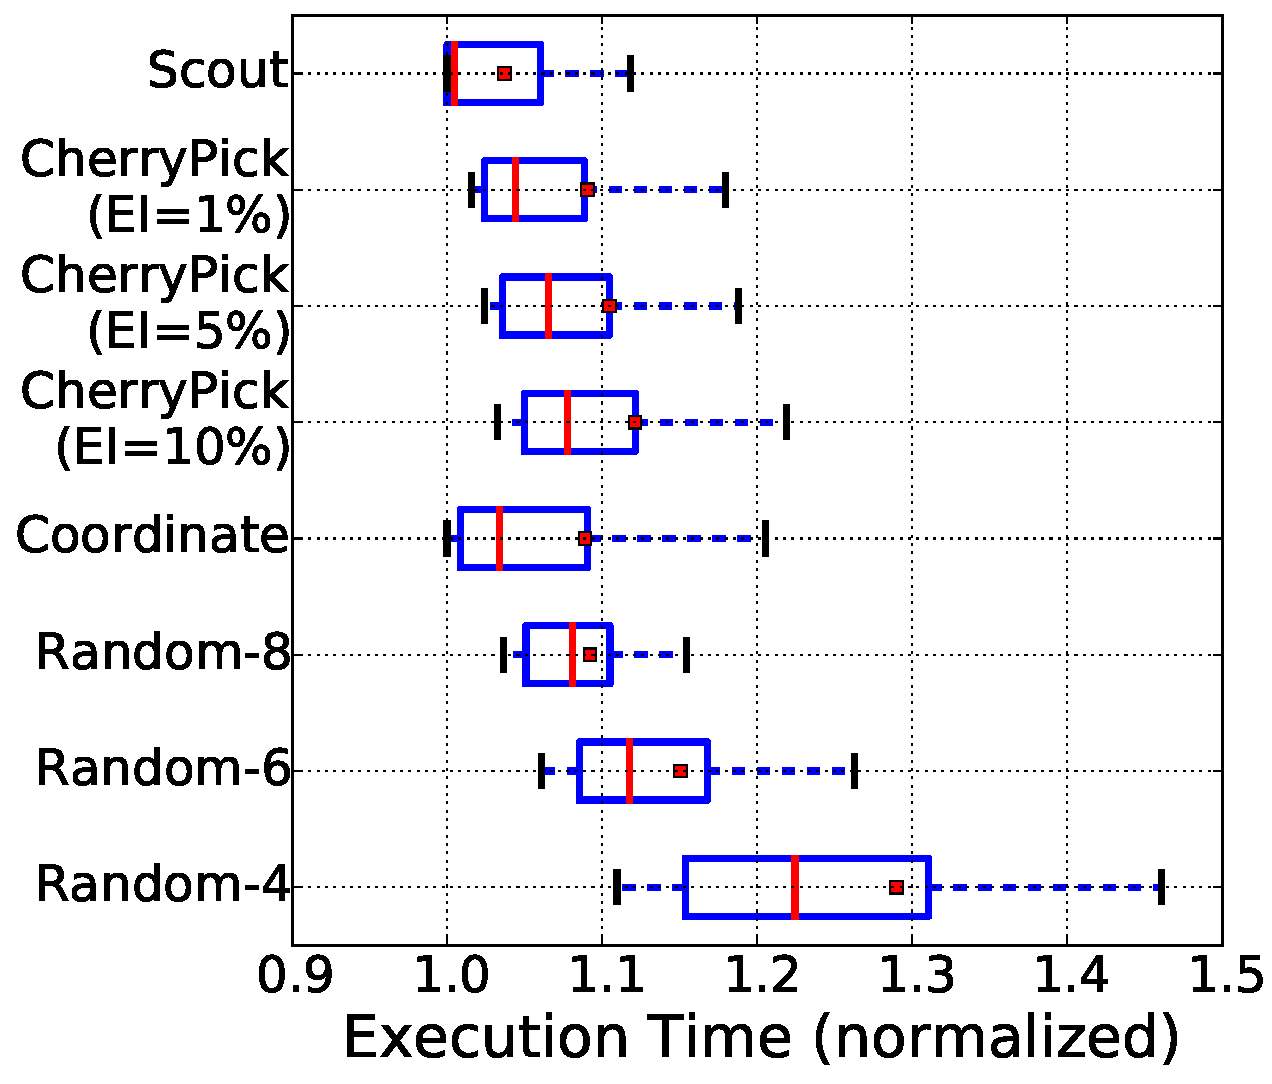
\includegraphics[width=\linewidth]{figures/single_time_overall_performance.pdf}
    \caption{Search Performance}
    \label{fig:single_time_overall_performance}
\end{subfigure}
\begin{subfigure}[b]{0.4\textwidth}
    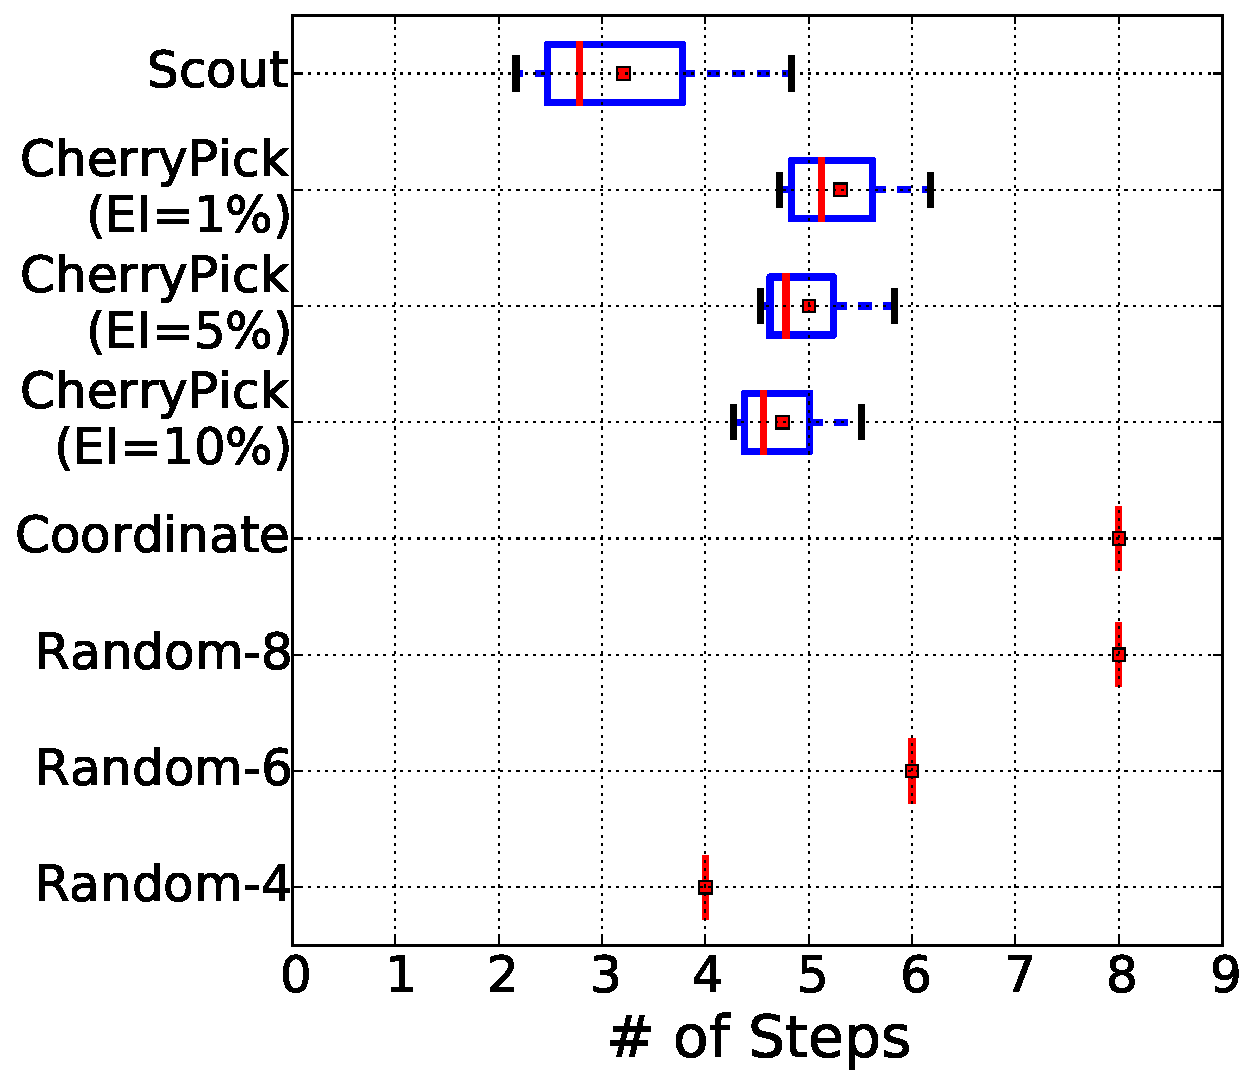
\includegraphics[width=\linewidth]{figures/single_time_overall_steps.pdf}
    \caption{Search Cost}
    \label{fig:single_time_overall_steps}
\end{subfigure}
\caption{\small{\textbf{Minimizing Execution Time.}
 The \emph{x-axis} represents the normalized performance (to the optimal configuration), and the optimal performance is $1$. 
 \scout finds the near-optimal solutions ($< 1.1$) in 87\% workloads while using much fewer steps.}}
\label{fig:single_time_overall}
\end{figure}


\subsubsection*{Deployment Choices}
Our evaluation examines both single- and multiple-node settings.
The single-node setting serves a comparison baseline and allows us to test more workloads (due to smaller search space).
In the single node setting,
we choose 18 distinct instance types or cloud configurations and 107 workloads.
When evaluating different cluster sizes,
we use strong scaling---fixed problem size---because we are interested in how to speed up a workload rather than the efficiency of the cluster.
For the multiple-node setting, we run 18 workloads
on 69 cloud configurations (9 instances with various cluster sizes).
%The search space is shown in~\myfigure{\ref{fig:search_space}}.

\subsubsection*{Dataset}
In order to verify the effectiveness of \scout,
we create a comprehensive performance data conversing all the combinations of
workloads and architectural configurations.
We collected our data on AWS.
\mytable{\ref{tab:dataset_overview}} present a summary.
Please refer to the open performance database for further details in Section~\ref{sec:cat::dataset}.


\subsubsection*{Parameters}
\scout has three important parameters:
1) labeled classes, 2) probability thresholds and 3) misprediction tolerance.
For the labeled classes in classification modeling,
we define five classes,
``better+'', ``better'',  ``fair'', ``worse'' and ``worse+'',
using thresholds [0.8, 0.95, 1.05, 1.2] as the cut points.
Regarding the two stopping criteria,
we choose $0.5$ for the probability threshold and
$3$ and $4$ for the misprediction tolerance
in the single-node and multiple-node setting respectively.
We examine the trade-off of these parameters in Section~\ref{sec:discussion}.

\subsection{Comparison Method}
To evaluate \scout, we examine the search performance
in terms of \emph{effectiveness}, \emph{efficiency} and \emph{reliability}.
We compare \scout with random search, coordinate descent, and \emph{CherryPick}.

\subsubsection*{Random search}
This search method
uniformly samples the configuration space.
The stopping criterion is the number of
configurations to evaluate.
A higher number yields better solution but also incurs higher search cost.
For a fair comparison, the search is repeated 100 times.  Random-4, -6, -8 represent random samples of 4, 6, and 8 cloud configurations respectively.
It serves as a na\"ive baseline method.


\begin{figure}[!htbp]
\centering
\begin{subfigure}[b]{0.4\textwidth}
    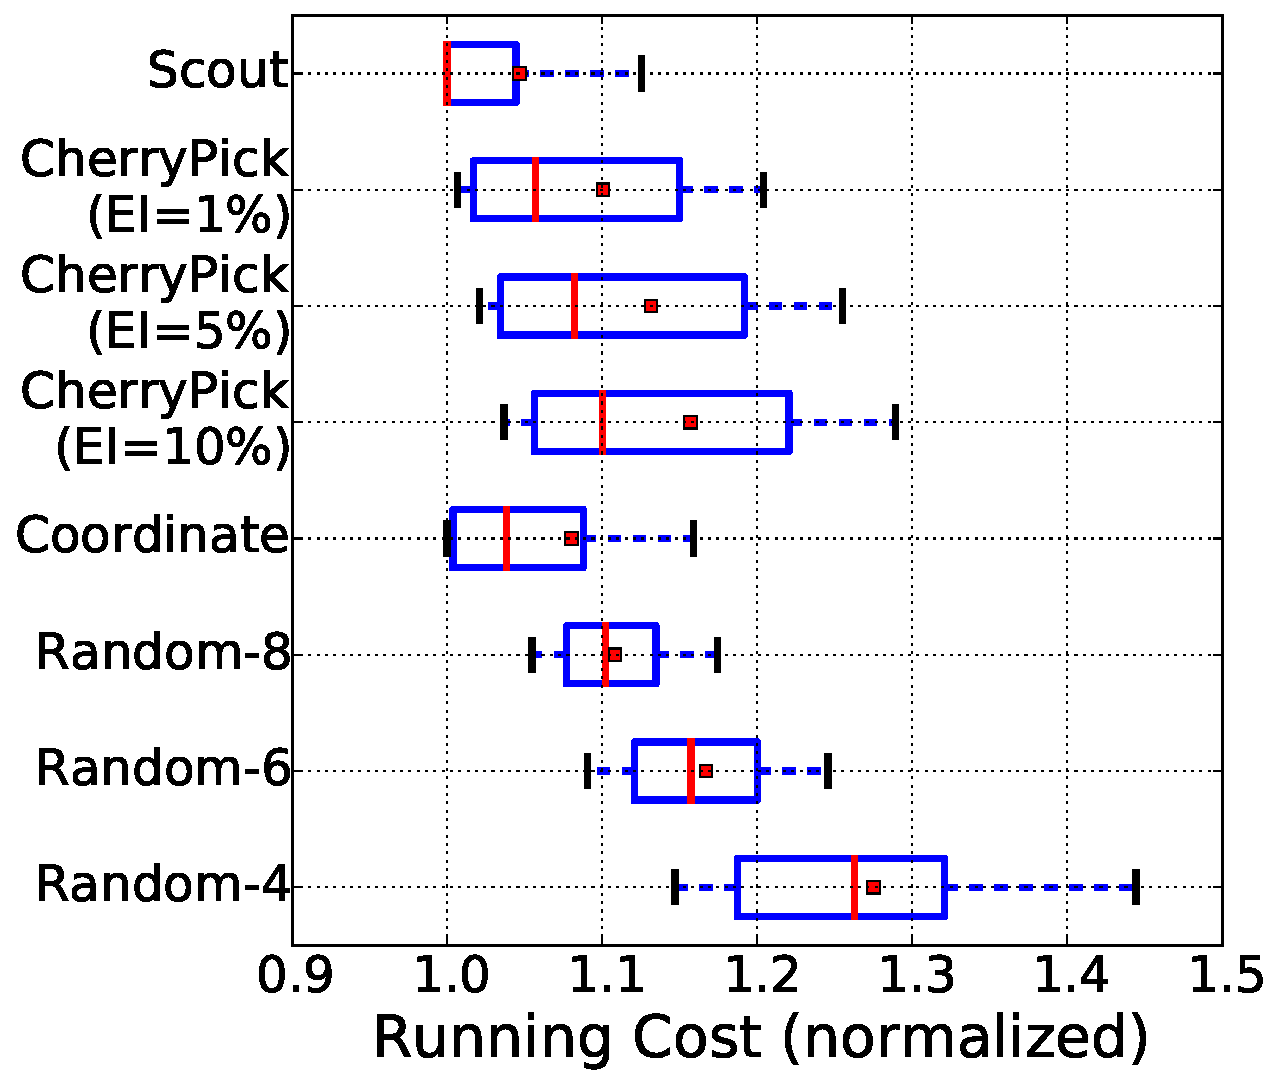
\includegraphics[width=\linewidth]{figures/single_cost_overall_performance.pdf}
    \caption{Search Performance}
    \label{fig:single_cost_overall_performance}
\end{subfigure}
\begin{subfigure}[b]{0.4\textwidth}
    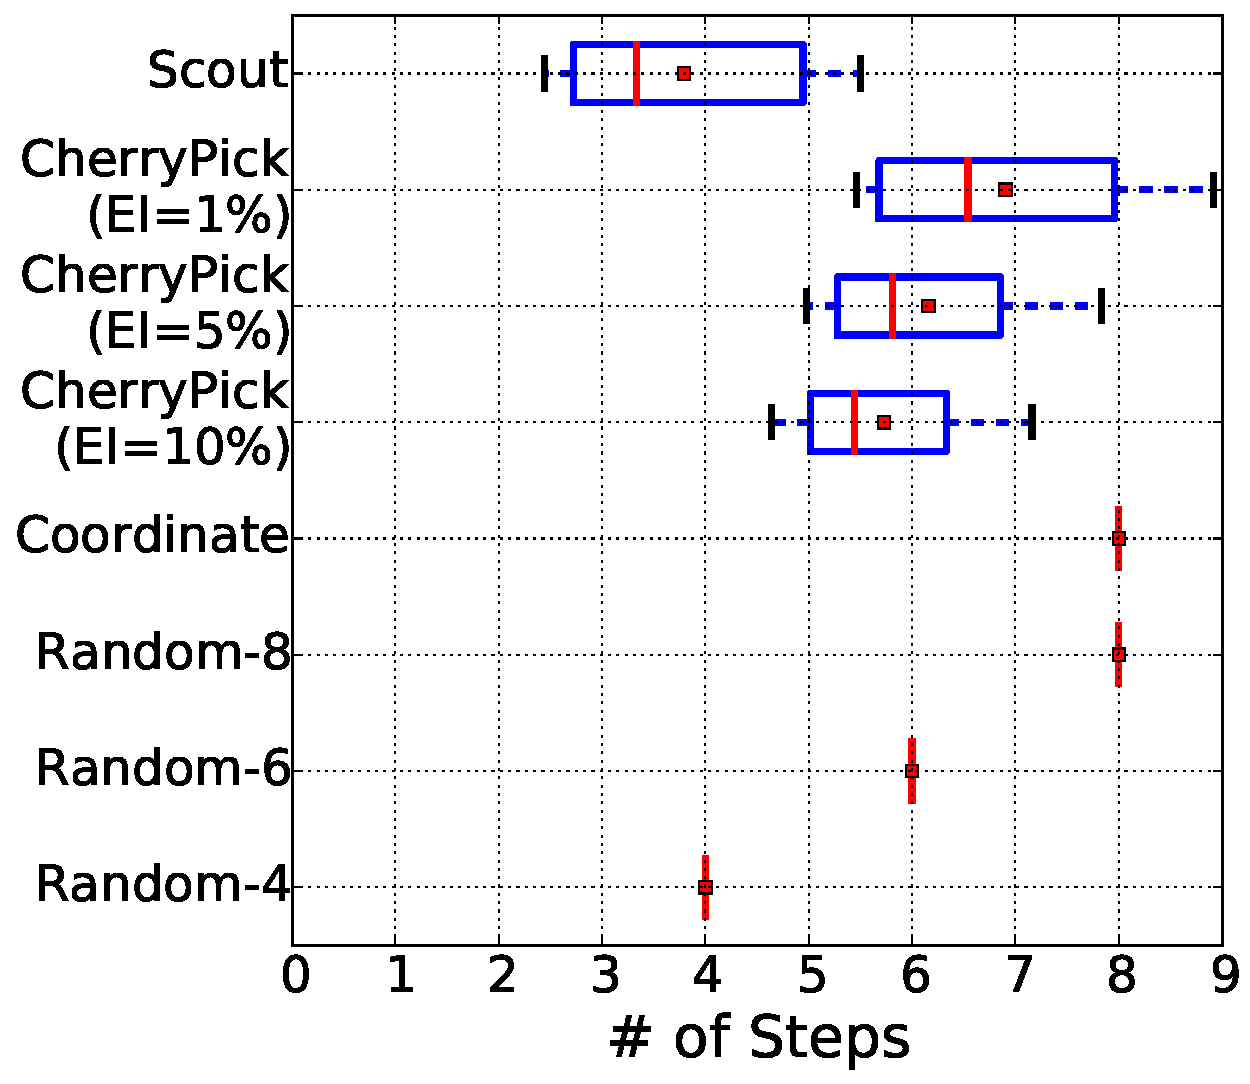
\includegraphics[width=\linewidth]{figures/single_cost_overall_steps.pdf}
    \caption{Search Cost}
    \label{fig:single_cost_overall_steps}
\end{subfigure}
\caption{\small{\textbf{Minimizing Running Cost.}
 Searching for the optimal cost is more difficult because the search cost is higher than the scenario of minimizing execution time. \scout still finds near-optimal solutions with a small increase in search cost while \emph{CherryPick} only finds near-optimal solutions in about 50\% workloads.}}
\label{fig:single_cost_overall}
\end{figure}


\subsubsection*{Coordinate descent}
This method searches
one dimension (\eg{CPU type and memory size}) at a time.
It determines the best choice of the dimension and
continues to choose the best from other dimensions.
This approach may suffer from local minimum due to
diminishing return and irregular performance outcome~\cite{Alipourfard2017}.
This situation worsens when the number of dimension increases.
In the evaluation, there are three dimensions:
(1) the instance family (such as \emph{c4} or \emph{r4}), (2)
the instance size (such as, \emph{large} or \emph{2xlarge}), and (3) the cluster size (the number of VMs).
The results are from 100 distinct searches, in which the starting point was randomly selected.


\subsubsection*{\cherrypick}
We implement the approach
proposed in \emph{CherryPick}~\cite{Alipourfard2017}.
We use
the same kernel function (\emph{Mat\'ern 5/2}) and
the same stopping criteria (\textbf{EI}=10\%).
We uniformly sample three configurations as starting points.
Since the search performance of \emph{CherryPick} is highly dependent on the selection of the starting points,
this experiment repeats 100 times to reduce artifacts
and give a better picture of \emph{CherryPick}'s capability.

We compare these approaches using three metrics.
First, we evaluate the effectiveness of the methods using
the \textit{normalized performance} (to the optimal choice).
It can be the \textit{execution time} or the \emph{deployment cost}.
Second, we use the search cost--- the number of cloud configurations measured to find the right cloud configuration.
% We consider the number of steps instead of the search cost (the total cost of actual measurements) because the former reveals how fast a method finds a solution.
Last, we examine how reliable our method is across the workloads. % (in single node setting) and 18 (in multiple-node setting).
We compare the aggregate of the normalized performance and the search cost along with their the 10\textsuperscript{th} and 90\textsuperscript{th} percentiles to observe whether our method performs well with consistency.  These numbers better illustrate reliability of the methods.


\begin{figure}[!htbp]
\centering
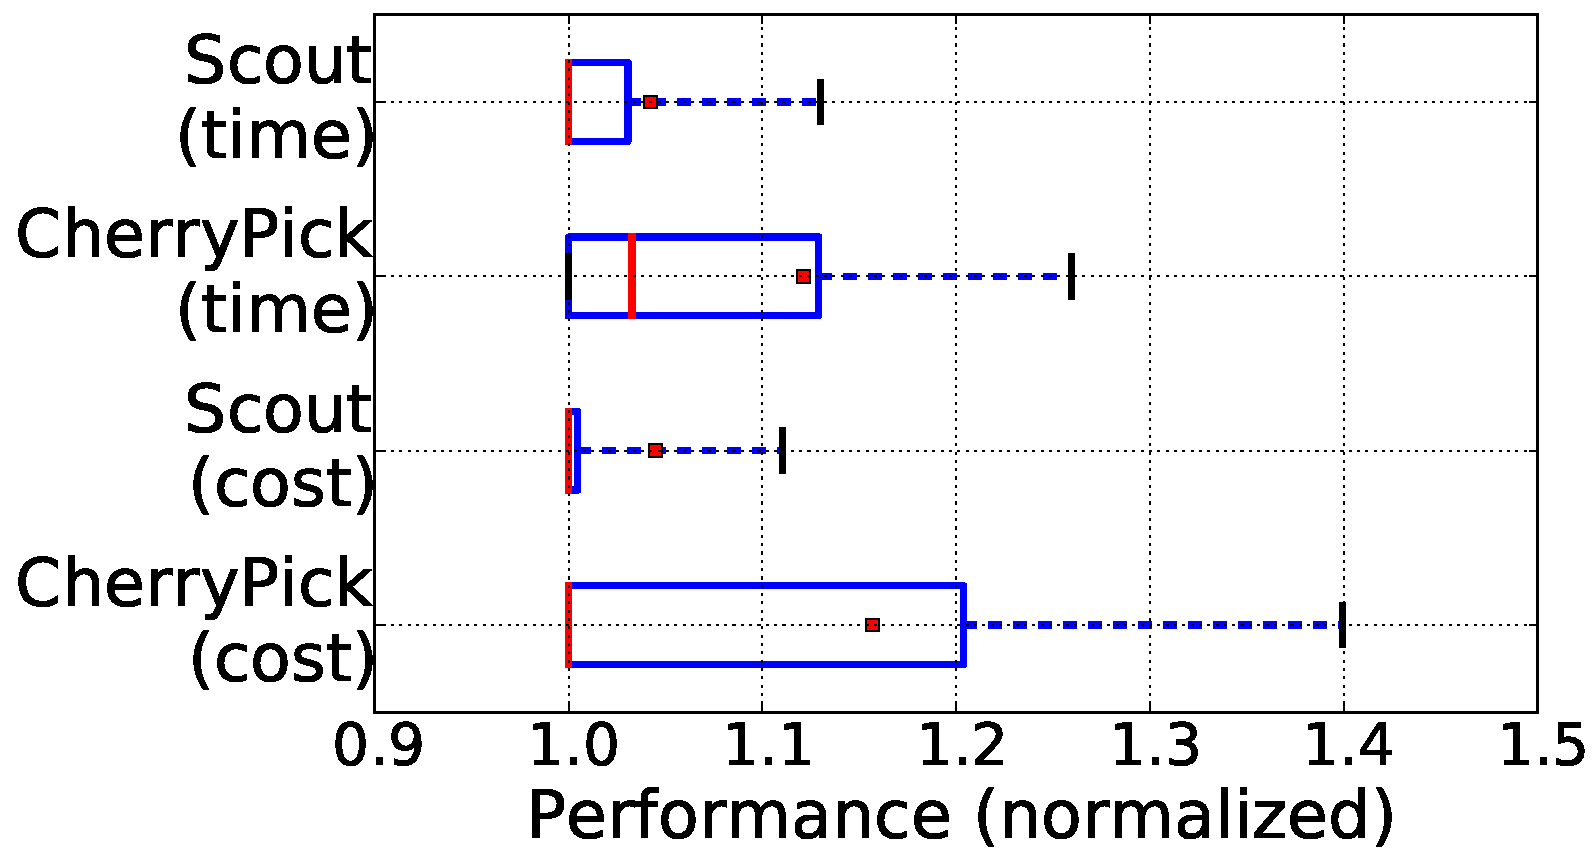
\includegraphics[width=0.6\textwidth]{figures/single_fragility.pdf}
\caption{\small{\textbf{Quality of found solutions.}
    Although both \emph{CherryPick} and \scout find the near optimal-solutions in most of the time,
    \scout is less fragile.}
}
\label{fig:single_fragility}
\end{figure}

\begin{figure}
\centering
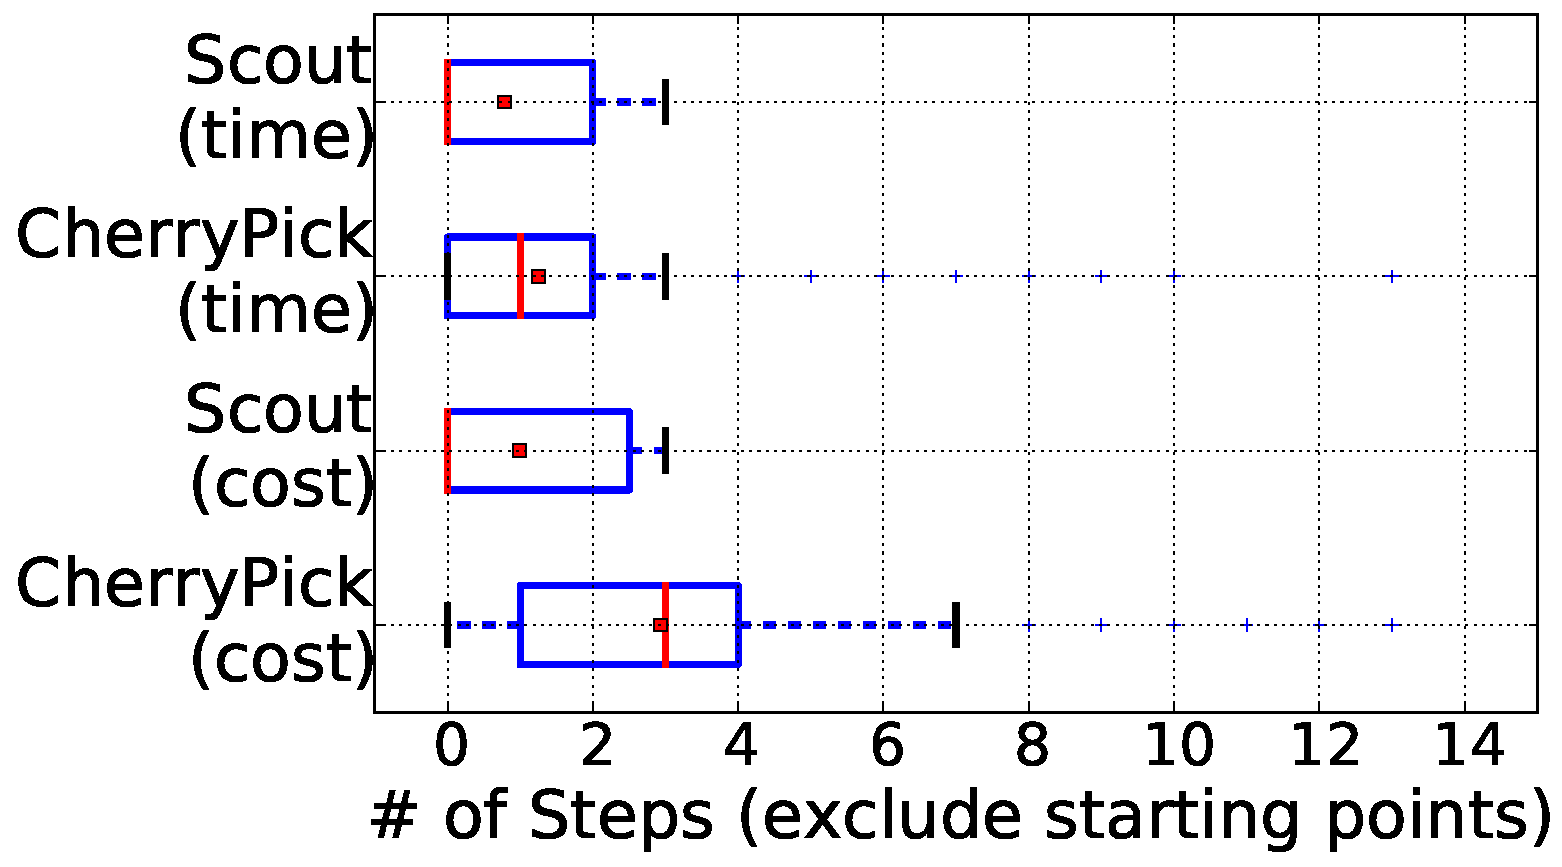
\includegraphics[width=0.6\textwidth]{figures/single_stopping_awareness.pdf}
\caption{\small{\textbf{Stopping awareness.}
    Search optimization avoids unnecessary search cost if it knows when the optimal solution is found.
    % \scout better acknowledges its existence.
    }}
\label{fig:single_startingpoint}

\end{figure}

\begin{figure}
\centering
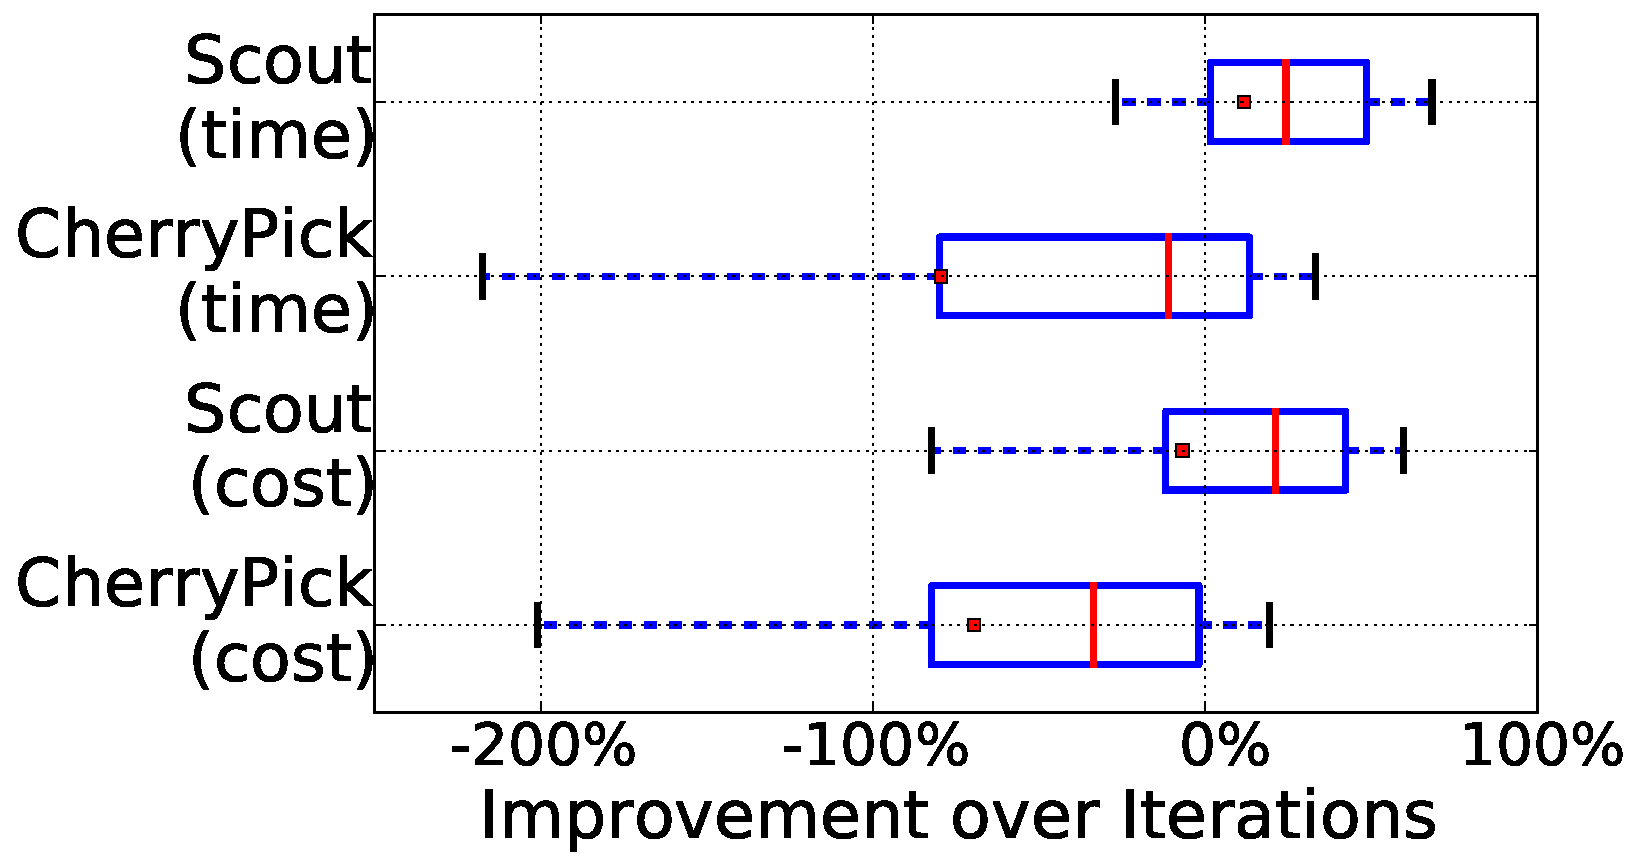
\includegraphics[width=0.6\textwidth]{figures/single_convergence.pdf}
\caption{\small{\textbf{Convergence speed.}
    \scout finds a better solution with 25\% improvement (on average) at each iteration, which suggests \scout is more likely to 
    converge.}}
\label{fig:search_convergence}
\end{figure}


\subsection{Is Scout effective and efficient?}

We examine search performance and search cost across 107 workloads in the single-node setting.
This evaluation largely answers whether a search method is reliable.

\textbf{Scout finds the near-optimal configurations
(within 10\% difference) for 87\% workloads}.
\myfigure{\ref{fig:single_time_overall_performance}} and \myfigure{\ref{fig:single_cost_overall_performance}} presents
the best cloud configuration (normalized to the optimal performance---1.0 represent the best, higher the worse) found by \scout and other methods while minimizing execution time and deployment cost, respectively. \myfigure{\ref{fig:single_time_overall_steps}} and \myfigure{\ref{fig:single_cost_overall_steps}} presents the search cost required the find the best cloud configuration which minimizes execution time and deployment cost, respectively. 
The figures display a box plot.
The box shows the inter-quartile range (from 25\textsuperscript{th} to 75\textsuperscript{th} percentile).
The vertical red line is the median, and the dot is the mean.
The whiskers to left and right show the 10\textsuperscript{th} and 90\textsuperscript{th} percentiles, respectively.
The horizontal axis shows execution time, and the vertical axis shows different techniques. 
An ideal search-based technique would find the best cloud configuration (in terms of performance) using the lower search cost.
These figures show the following.

\begin{itemize}[leftmargin=*]
    %\setlength\itemsep{-0.4em}
    \item \scout finds the best relative performance in terms of both execution time and deployment cost. The median performance of \scout, while searching for the cloud configuration which minimizes the deployment cost is 1.0, which means \scout was able to find the right cloud configuration.
    \item \scout is better than CherryPick across all measures (execution time, deployment cost, and search cost).
    \item \scout finds the best relative performance using the least search cost (fewer number of steps). Random-4 also requires low search cost, but its performance is much worse than \scout.
    \item The variance in the performance (in terms of execution time and deployment cost) of \scout is much lower than the other methods. The large variance of the Random methods can be attributed to their inherent randomness.
\end{itemize}


Overall, we see that \scout is that best performing method and \emph{CherryPick}, the state of the art method, only delivers similar performance in 64\% workloads while requiring 47\% greater search cost (4.7 compared to 3.2 steps). We also observe that the variance in the best cloud configuration found by \scout over 100 runs across 107 workloads is much lower than the other method. Hence, we can conclude that \scout is a reliable method to find the best cloud configuration.

\noindent\textbf{Cost creates a level playing field.}
Optimizing execution time is relatively easy
because a larger, more powerful instance type is more likely to have a shorter execution time.
However, the more powerful types are more expensive to execute.
Consequently, a smaller instance type may run longer but cost less.
Because the cost to execute an instance grow as the raw hardware performance increase, the differences in deployment cost between configurations tend to be much less than the differences between execution time.
This levels the playing field for cost---many more configurations are good candidates.
This leveling leads to, in general, longer searches,
as shown in \myfigure{\ref{fig:single_cost_overall_steps}}.
\emph{CherryPick} requires one extra step in optimizing deployment cost with a 15\% decrease of workloads in which it fails to find a solution within 10\% of the optimal configuration. To summarize, the performance of a search-based method is dependent on the objective of the search. From the data, we observe that searching for the best cloud configuration in terms of cost is more challenging than finding the best cloud configurations in terms of execution time. 




\subsection{Is \scout reliable?}
Users are willing to use a tool only when it is reliable. We evaluate the performance of \emph{CherryPick} and \scout
with different initial points for understanding their consistency.
In BO in \emph{CherryPick}, uses a random initial points to seed the search process and the effectiveness of CherryPick depend on these initial points. Selecting these initial points is non-trivial because (1) a good set of starting points for one workload does not work for other workloads, and (2) cloud providers frequently upgrade their instance portfolio with new instance types which make the process of selecting initial points more challenging. \scout is robust such that the effectiveness of \scout does not rely on initial points.


\begin{figure}[!htbp]
\centering
\begin{subfigure}[b]{0.4\textwidth}
    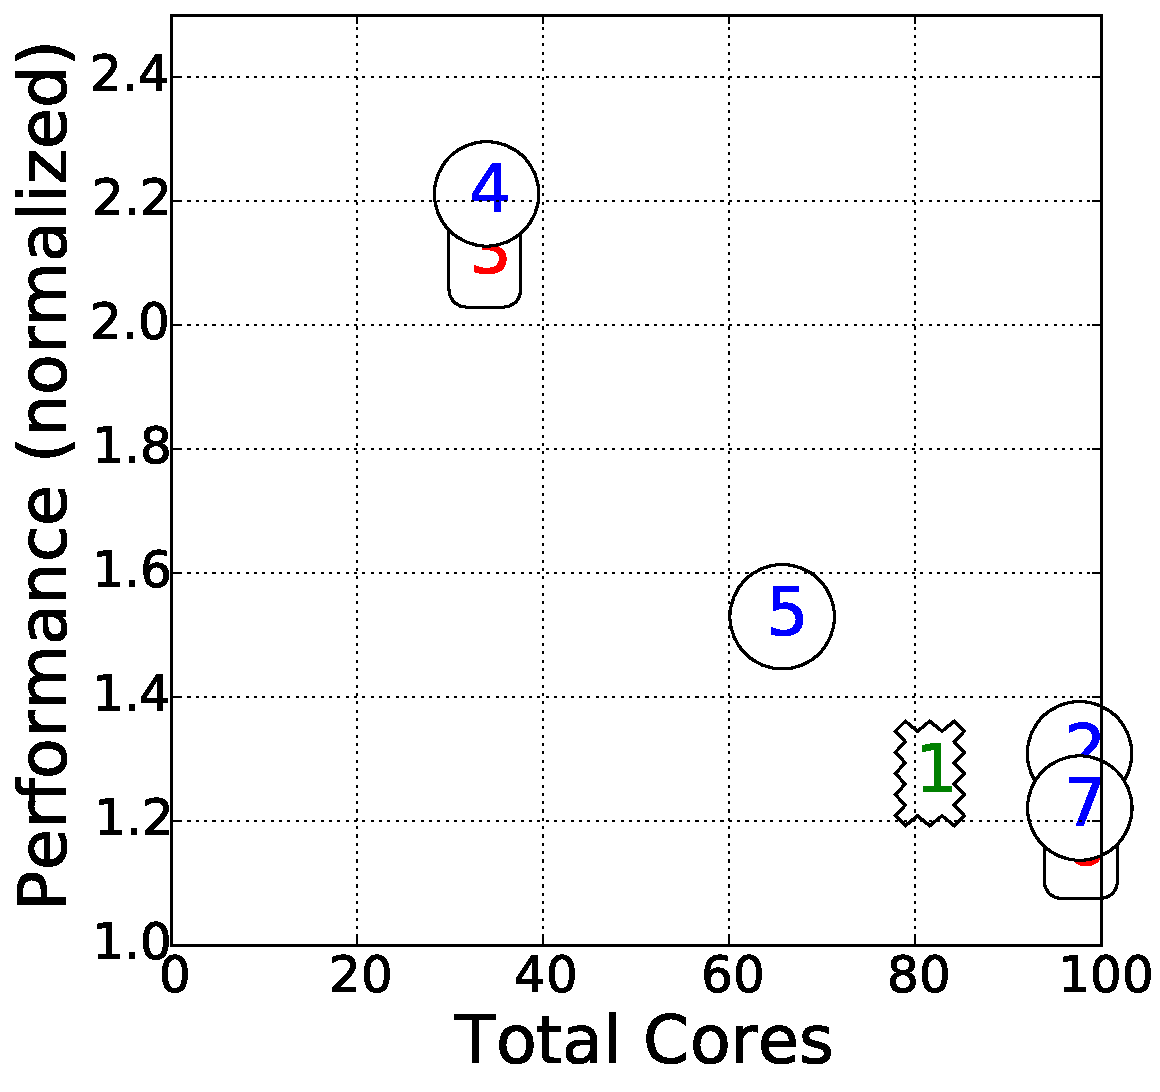
\includegraphics[width=\linewidth]{figures/multiple_bo_time_hadoop.pagerank.bigdata_12_cores.pdf}
    \caption{\cherrypick}
    \label{fig:comparison_time_cherrypick}
\end{subfigure}
\begin{subfigure}[b]{0.4\textwidth}
    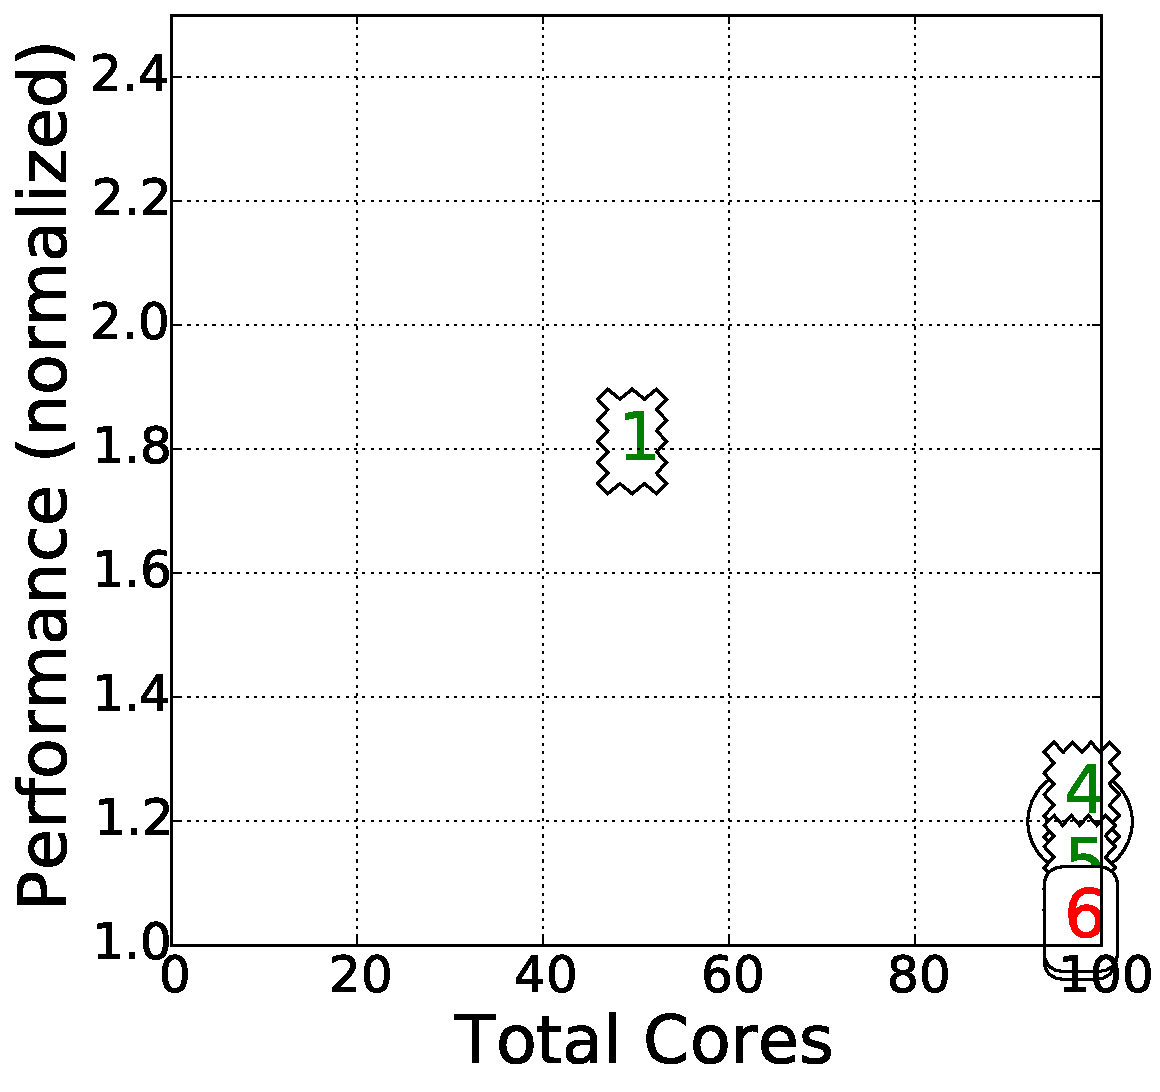
\includegraphics[width=\linewidth]{figures/multiple_scout_time_hadoop.pagerank.bigdata_24_m4.large_cores.pdf}
    \caption{\scout}
    \label{fig:comparison_time_scout}
\end{subfigure}
 \caption{\small{\textbf{Finding the fastest configuration for PageRank on Hadoop.} Left \& right sub-figure show the search path of CherryPick and \scout respectively. \scout identifies PageRank as a compute-intensive workload.  It chooses the configurations with higher core counts and CPU speed.}}
\label{fig:compare_1}
\end{figure}


To demonstrate the robustness of \scout, for each workload, we varied the initial points used in \emph{CherryPick}.
These points were randomly (without replacement) selected from the search space. On the other hand, \scout only needs one starting point, which is also selected randomly. This experiment was repeated 100 times to understand the implication of randomness.
\myfigure{\ref{fig:single_fragility}} shows the variance in the normalized performance of the found solutions by both the methods.
We see that 

\begin{itemize}[leftmargin=*]
    %\setlength\itemsep{-0.4em}
    \item \scout can find the optimal cloud configuration for most of the case since median performance is 1.0. However, there are some outliers which pushes the mean to 1.05. This is not a major concern since the 75$^{th}$ percentile is less than 1.05. This goes to show that the variance in the performance of 107 workloads aggregated over 100 runs is low.
    \item CherryPick is also effective in finding the cloud configuration since its median performance over 107 workloads is 1.05. We notice that the variance of the performance (both in terms of search performance and time) is larger than \scout. 
\end{itemize}


The variance in the results of CherryPick can be a major concern for the practitioners since a bad choice of initial points can lead to selecting either a slow or expensive configurations.
\scout, on the other hand, has more stable search performance regardless of the starting point.


\subsection{Why \scout works better?}
\label{sec:why_better}

\scout relies on quality routing policy to deliver good solutions.
We find \scout effective because
it knows when to stop searching and
converges to better solutions.

\begin{itemize}
\item \textbf{\scout knows when to stop.}
When an optimizer can stop as soon as it finds the optimal solution (or near-optimal solutions),
it can avoid unnecessary search efforts. \myfigure{\ref{fig:single_startingpoint}} shows that \scout requires a fewer number of steps if the starting point is already the optimal configuration.

\item \textbf{Convergence speed.}
The speed of convergence of a search-based method is dependent how it selects the next cloud configuration to measure. An ideal search-based method will always find the next cloud configuration, which is better than the cloud configurations sampled previously. \textit{Converge speed} can be defined as the average difference between the performance score (execution time or deployment cost) of the previous measurement (i$^{th}$ step) and the current measurement (i+1$^th$ step). A positive number would indicate that the current cloud configuration is better than the previous measurement (for both deployment cost and execution time, lower is better). \myfigure{\ref{fig:search_convergence}} compares the convergence speed of CherryPick and \scout. \myfigure{\ref{fig:search_convergence}} indicates that \scout overall finds cloud configurations 50\% (median) better execution time than the current cloud configuration, whereas CherryPick overall moves to cloud configuration which is 25\% worse than the current best configuration. Similar behavior is seen for deployment cost. This is evidence to show that \scout uses the historical data to find the promising region in the search space and exploits that space effectively.

\end{itemize}



\begin{figure}[!htbp]
\centering
\begin{subfigure}[b]{0.4\textwidth}
    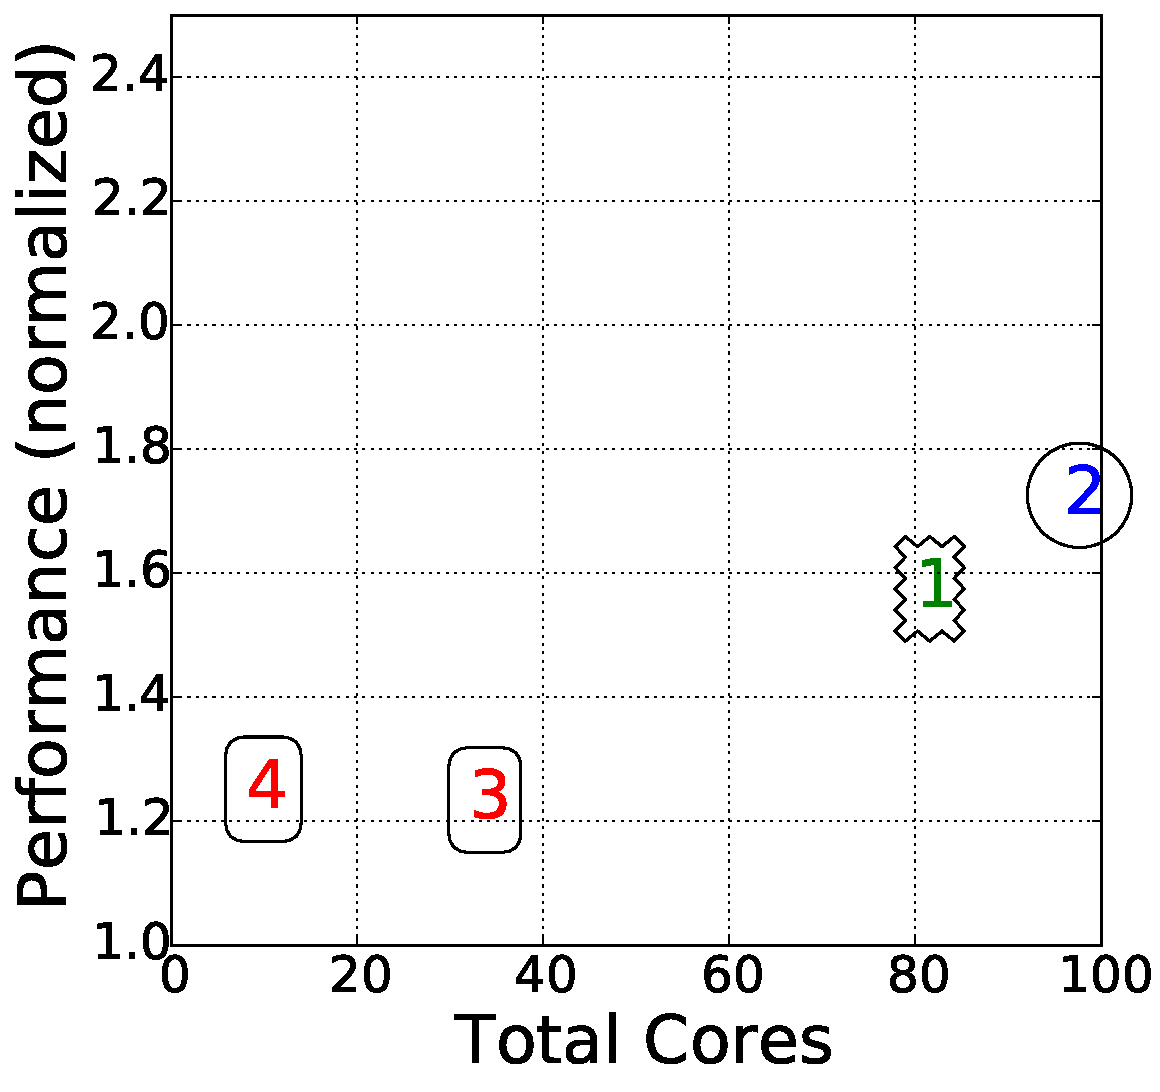
\includegraphics[width=\linewidth]{figures/multiple_bo_cost_spark1.5.naive-bayes.huge_12_cores.pdf}
    \caption{\cherrypick}
    \label{fig:comparison_cost_cherrypick}
\end{subfigure}
\begin{subfigure}[b]{0.4\textwidth}
    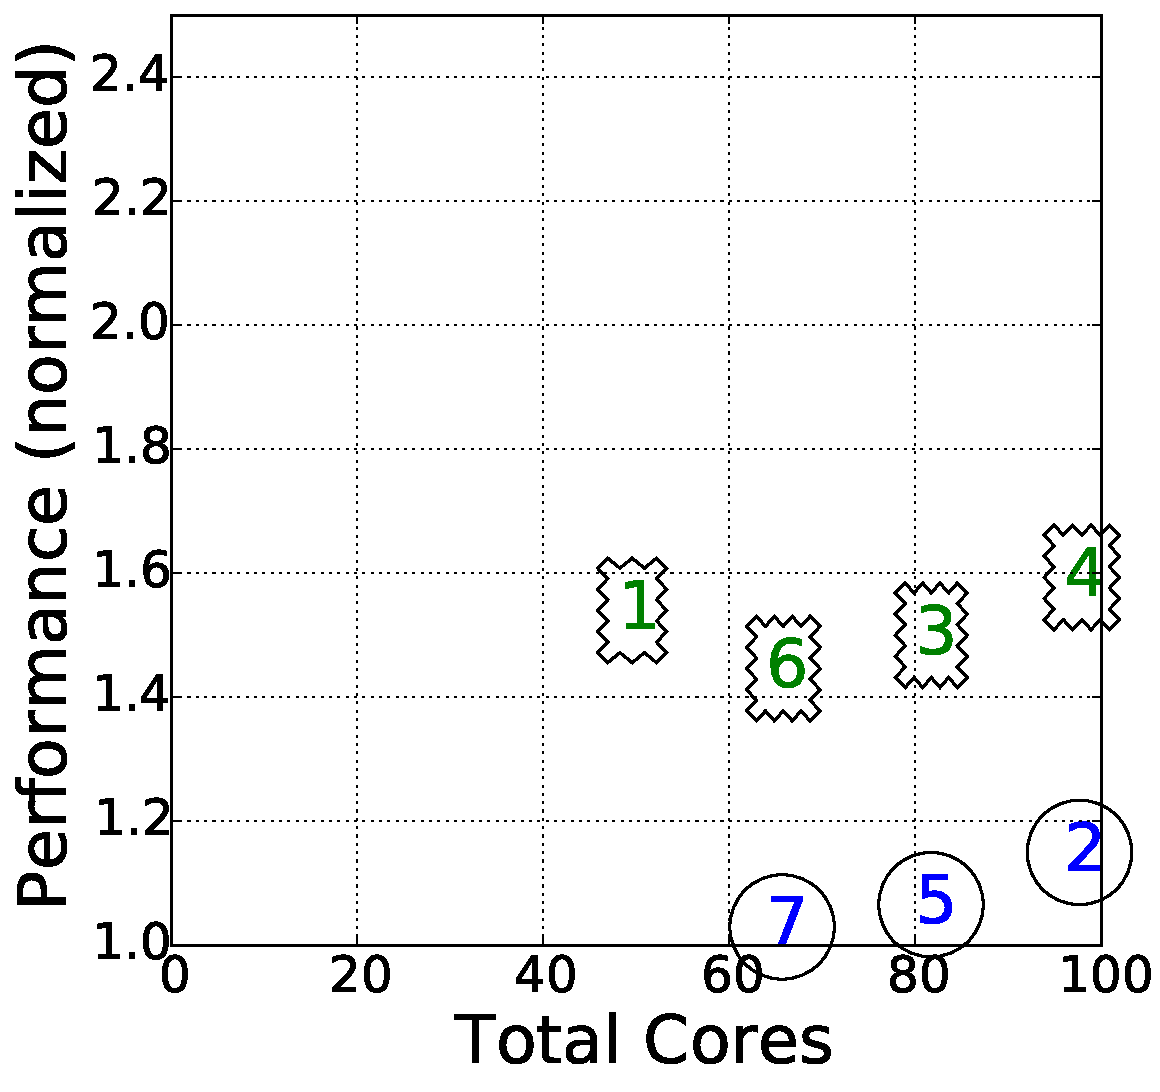
\includegraphics[width=\linewidth]{figures/multiple_scout_cost_spark1.5.naive-bayes.huge_24_m4.large_cores.pdf}
    \caption{\scout}
    \label{fig:comparison_cost_scout}
\end{subfigure}
\caption{\small{\textbf{Minimizing the running cost for Naive-Bayes on Spark.} This is a memory-intensive workload.  \scout does not even try the \emph{c4} family due to its small memory per core.}}
\label{fig:compare_4}
\end{figure}



\subsection{Example Search Process}

This section compares and contrasts the properties of \emph{CherryPick} and \scout.
We provides four examples of optimizing execution time (in Figure~\ref{fig:compare_1} and~\ref{fig:compare_2}) and running cost (in Figure~\ref{fig:compare_3} and~\ref{fig:compare_1}). Different colored markers in the graphs represent different families of instances: \textcolor{green}{green} represent the m4 family---general purpose, \textcolor{blue}{blue} represent the r4 family---memory optimized, and \textcolor{red}{red} represent the c4 family---compute optimized.
We evaluate \emph{CherryPick} and \scout on four representative workloads, selected based on diverse resource requirements (CPU intensive, Memory intensive).
For \emph{CherryPick}, we choose
\emph{20$\times$m4.xlarge}, \emph{48$\times$r4.large} and \emph{16$\times$c4.large} as the starting points because
they are wide spread in the search space.
Since \scout only needs one starting point,
we choose \emph{24$\times$m4.large} because it is the mid point of the search space.
We observe that \emph{CherryPick} can find near-optimal solutions for few workloads if not all.

\begin{figure}[!htbp]
\centering
\begin{subfigure}[b]{0.4\textwidth}
    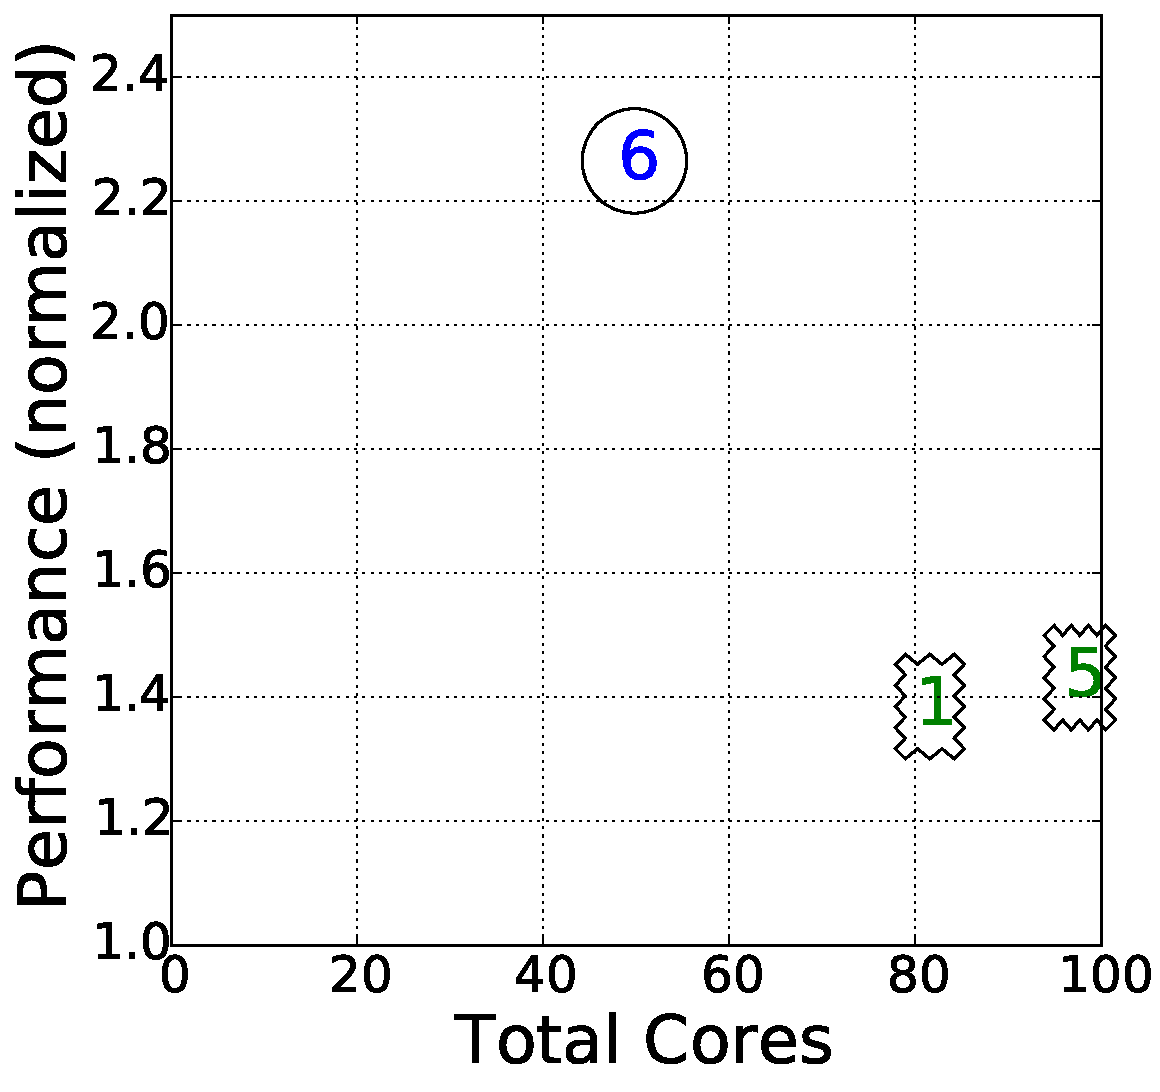
\includegraphics[width=\linewidth]{figures/multiple_bo_time_spark1.5.regression.huge_12_cores.pdf}
    \caption{\cherrypick}
    \label{fig:search_time_cherrypick}
\end{subfigure}
\begin{subfigure}[b]{0.4\textwidth}
    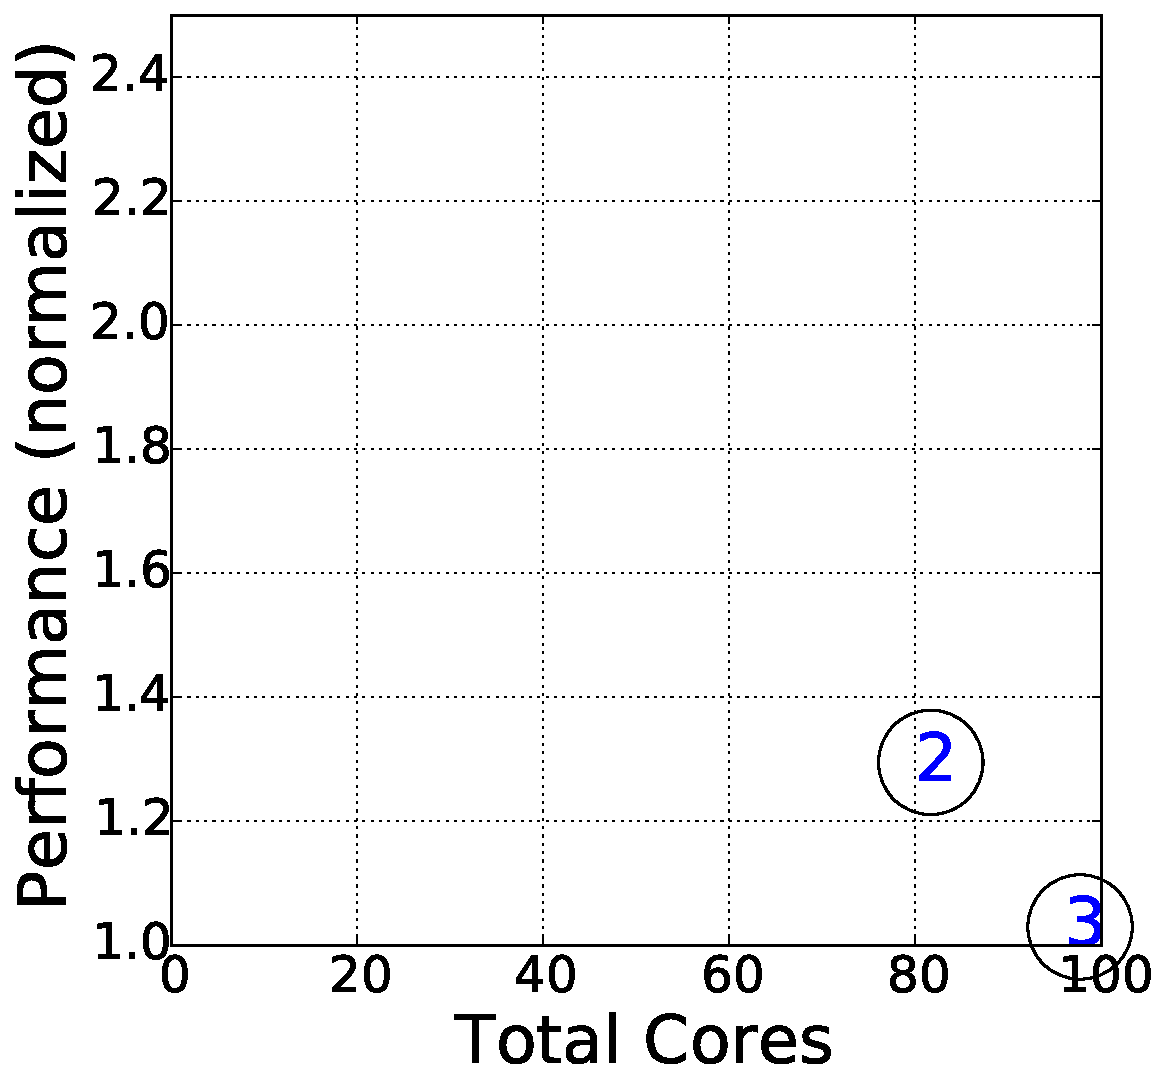
\includegraphics[width=\linewidth]{figures/multiple_scout_time_spark1.5.regression.huge_24_m4.large_cores.pdf}
    \caption{\scout}
    \label{fig:search_time_scout}
\end{subfigure}
\caption{\small{\textbf{Minimizing execution time of Regression on Spark.} Since the Regression workload requires both computation and large memory, \scout directly chooses configurations with the \emph{r4} family and larger cores.}}
\label{fig:compare_2}
\end{figure}

\subsubsection*{Reliable exploration is difficult and generates high search cost}
In Figure~\ref{fig:compare_2},~\ref{fig:compare_3},~\ref{fig:compare_1},~\ref{fig:compare_4}, we observe that the search path generated by \emph{CherryPick} involves more distinct VM types due to the need to explore the performance model. For example, in Figure~\ref{fig:compare_3}, CherryPick visits each instance family at once in all examples while \scout skips some specific families.
This is because \scout builds the performance model from historical data. Hence, it requires only little (or no) exploration. This phenomenon, exploration-exploitation dilemma, is studied extensively in Machine learning~\cite{kaelbling1996reinforcement}. The cold-start issue (as described in Section~\ref{sec:motivation} arises partly because of the requirement to explore the configuration space since \scout learns the performance behavior from historical data from workloads (previously explored) can sidestep the need to explore the search space.




\subsubsection*{Fragility of CherryPick}
As explained in Section~\ref{sec:motivation}, CherryPick is fragile
because it is sensitive to its parameters and the starting points.
In the four examples, \emph{CherryPick} starts from the same three configurations; however, the results are very different.
In \myfigure{\ref{fig:compare_3}}, \emph{CherryPick} fails to characterize the search space, which results in long search path (and high search cost).
While in \myfigure{\ref{fig:compare_4}},
\emph{CherryPick} stops too early and only finds a local minima (the $c4$ family).
These two examples show that \emph{CherryPick} is fragile and therefore, its search performance is not stable.

\subsubsection*{\scout identifies resource requirements}
When resource requirements can be articulated, a search process is more likely to find cloud configurations effectively and efficiently. In \myfigure{\ref{fig:compare_1}},
the \emph{PageRank} workload runs faster on a larger cluster (higher core counts) and higher-frequency CPUs. The \emph{r4} family, with larger memory but slower CPU speed, does not seem to be the best choice, hence avoided by \scout and instead prefers \emph{c4} and \emph{m4} family.
This tendency is more clear in the other cases as well (Figure~\ref{fig:compare_2}, ~\ref{fig:compare_3}, and~\ref{fig:compare_4}).


\begin{figure}[!htbp]
\centering
\begin{subfigure}[b]{0.4\textwidth}
    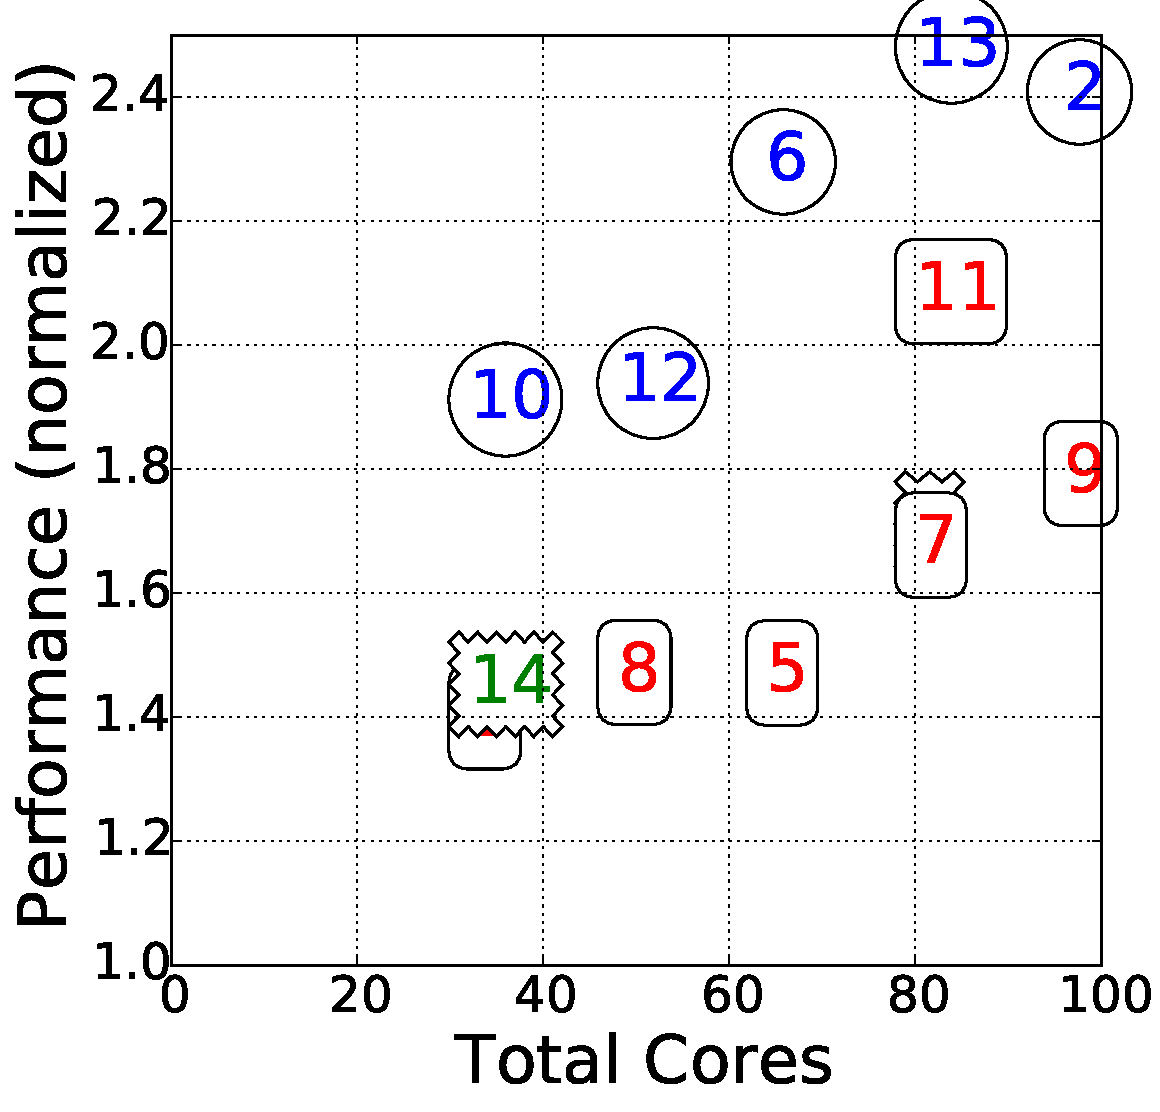
\includegraphics[width=\linewidth]{figures/multiple_bo_cost_hadoop.terasort.bigdata_12_cores.pdf}
    \caption{\cherrypick}
    \label{fig:search_cost_cherrypick}
\end{subfigure}
\begin{subfigure}[b]{0.4\textwidth}
    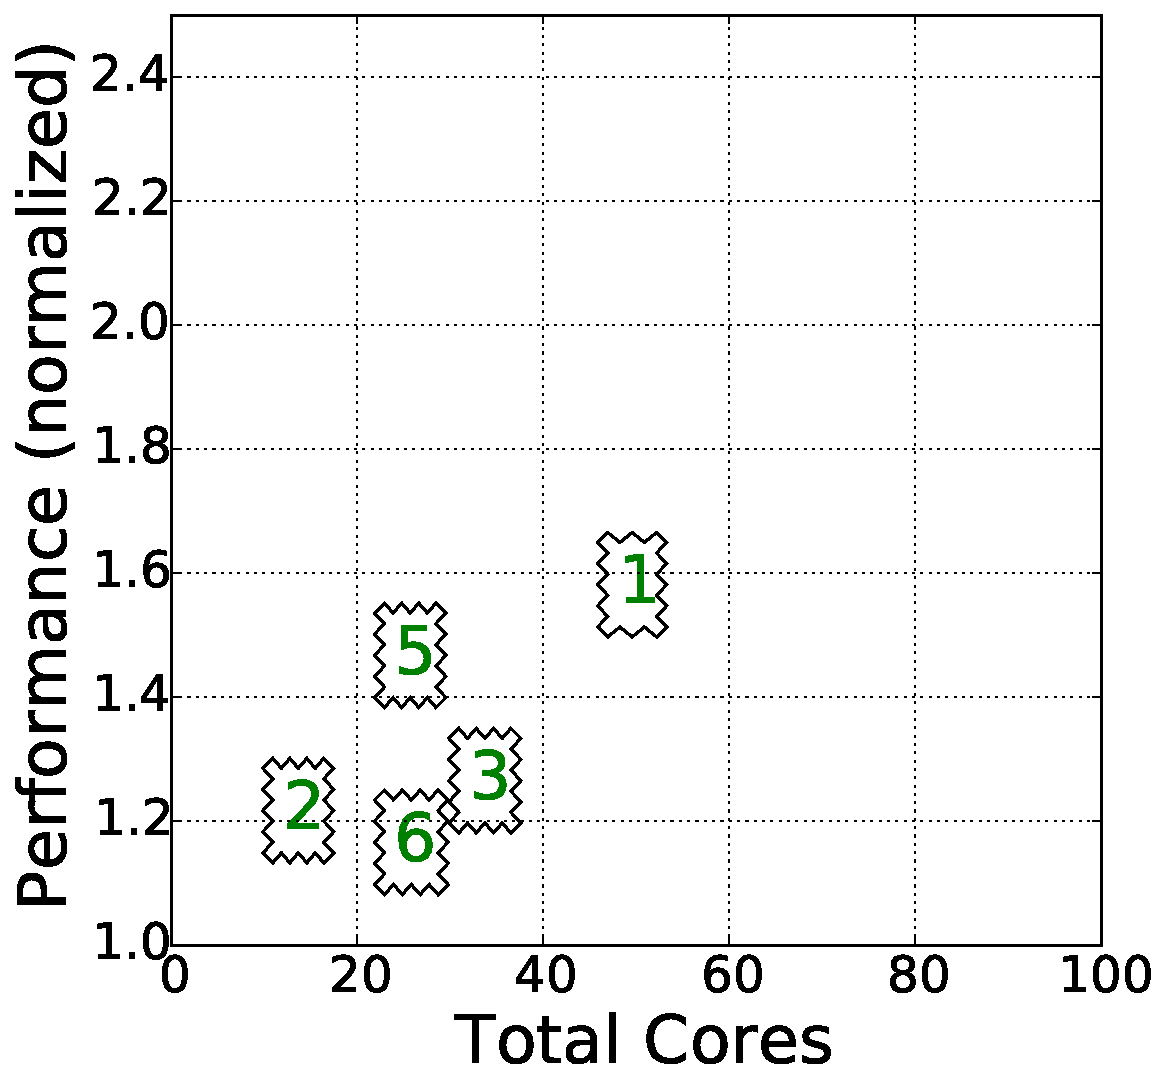
\includegraphics[width=\linewidth]{figures/multiple_scout_cost_hadoop.terasort.bigdata_24_m4.large_cores.pdf}
    \caption{\scout}
    \label{fig:search_cost_scout}
\end{subfigure}
\caption{\small{\textbf{Finding the cheapest configuration for Terasort on Hadoop.} The Terasort workload requires enough memory to avoid spilling data to disks. Besides, a large cluster can be insufficient due to the shuffle phase in MapReduce.  \scout chooses a smaller cluster with the general-purpose VM type. }}
\label{fig:compare_3}
\end{figure}



\subsubsection*{\scout captures the complex cost model}
In a real-world setting, practitioners can choose either a smaller cluster built using more powerful instances or choose large cluster built using smaller or less powerful instances (a scale-out and a scale-out configuration). The performance model used by \scout can infer the size of the cluster of the best cloud configuration.
In \myfigure{\ref{fig:compare_3}}, \scout chooses to run \emph{TeraSort} on a smaller cluster to save cost. On the contrary, in Figure~\ref{fig:compare_4}, \scout selects a larger cluster for efficiently running the \emph{Naive-Bayes} workload while achieving lower cost. These two examples show that \scout captures the complex relationship between the resource metrics and the running cost.


\subsubsection*{Summary}
The main difference between \emph{CherryPick} and \scout lies how the method explores the space of possible cloud configuration options. We can see that \emph{CherryPick} has to explore more cloud configuration options and hence have higher search cost (longer search path) while \scout searches within a relatively restricted region. This feature of \scout can be attributed to its performance model, which learns from the historical data. This also goes to show that encoding scheme, which uses low-level performance metrics, is successful in transferring knowledge from one workload to another.



\section{Discussion}
\label{sec:discussion}


\subsection*{Tuning Searching Performance}

\scout uses ``probability threshold'' and ``misprediction tolerance'' as stopping criteria.
%We examine how they affect the search performance of \scout.\\

\subsubsection*{Probability Threshold}
\scout chooses the next configuration to evaluate
based on the probability of improvement and
stops when the probability is lower than the probability threshold $\alpha$.
\myfigure{\ref{fig:single_probability_threshold}} shows that
a higher probability threshold is pessimistic and 
terminates the search process prematurely,
hence, shorter search path
and unstable search results). 
The probability threshold presents a trade-off between
search performance and search cost.
The right threshold must consider
the reliability curve of classification methods~\cite{niculescu2005predicting}.

\subsubsection*{Misprediction Tolerance}
\scout terminates the search process if the selected configurations do not improve the current best choice (considered as a misprediction).
\scout maintains a counter of mispredictions.
A higher limit tolerates more mispredictions but yields better search performance due to more chances.
A proper limit should consider both
the size of search space and the accuracy of prediction.
In \myfigure{\ref{fig:single_misprediction_tolerance}},
we show that a higher tolerance level leads to better search performance but higher search cost.
This trade-off is similar to the probability threshold.

\begin{figure}[!htbp]
\centering
\begin{subfigure}[b]{0.4\textwidth}
    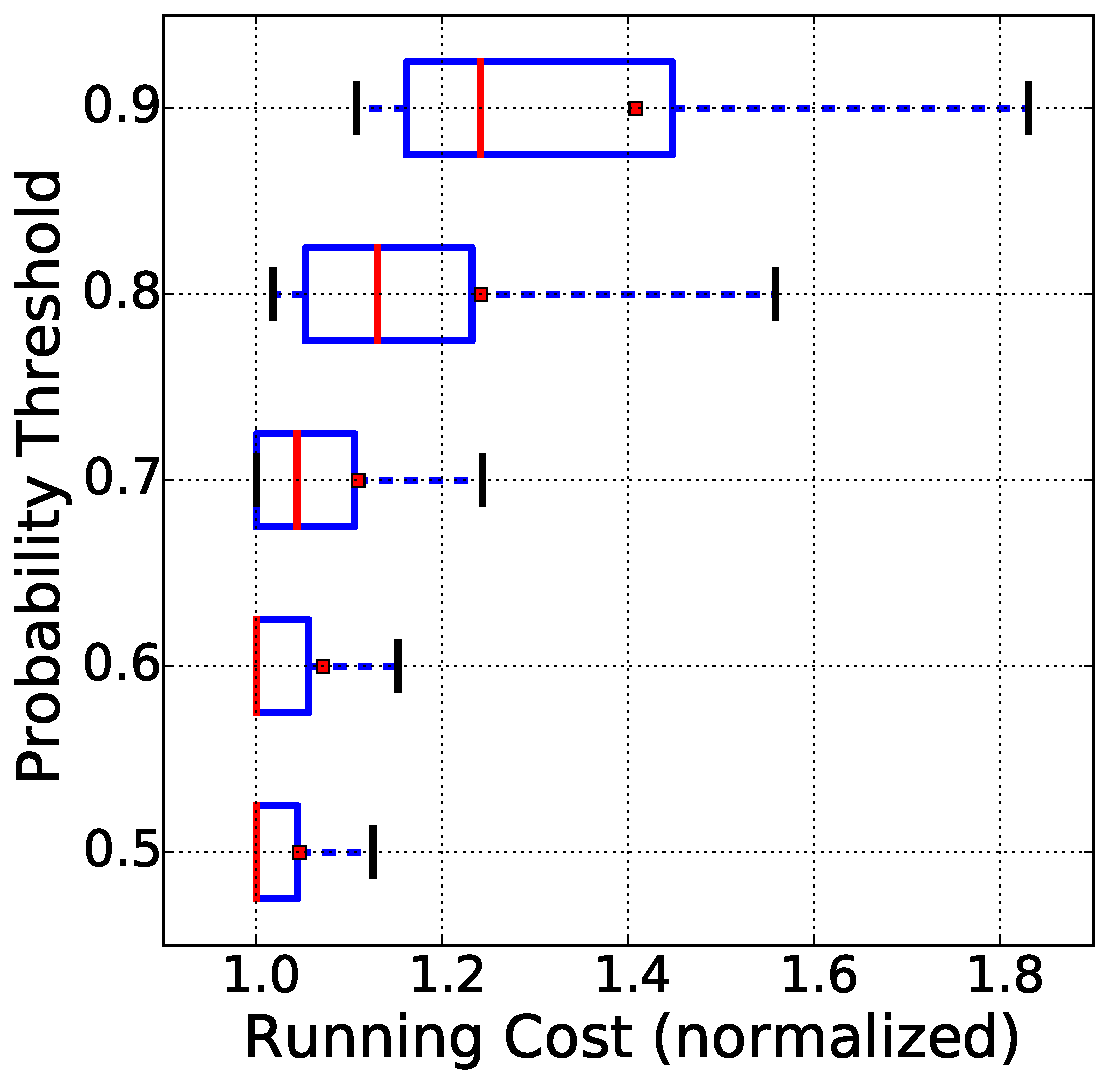
\includegraphics[width=\linewidth]{figures/single_cost_tuning_probability_performance.pdf}
    \caption{Search Performance}
    \label{fig:single_cost_tuning_threshold_performance}
\end{subfigure}
\begin{subfigure}[b]{0.4\textwidth}
    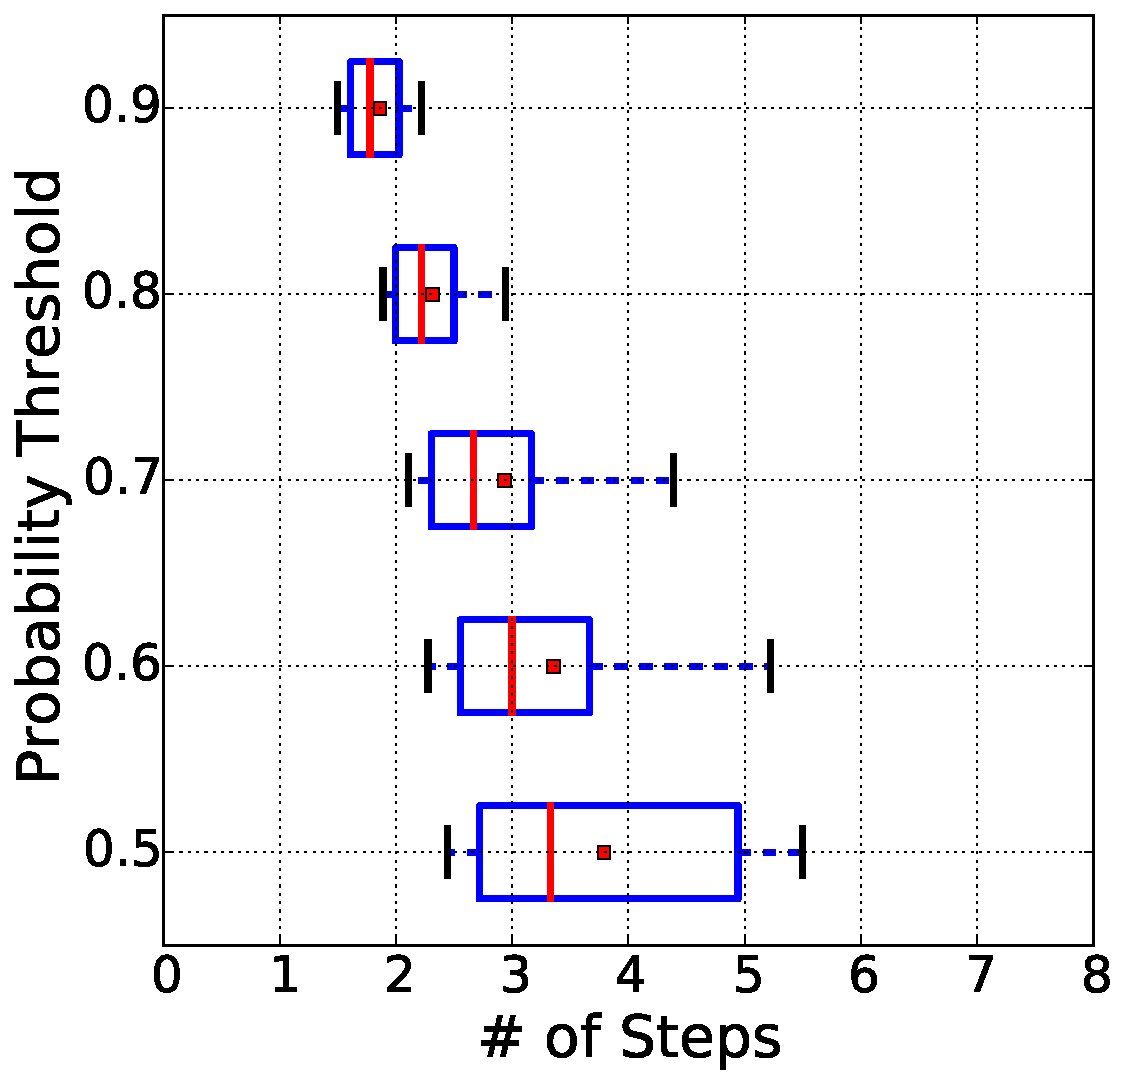
\includegraphics[width=\linewidth]{figures/single_cost_tuning_probability_steps.pdf}
    \caption{Search Cost}
    \label{fig:single_cost_tuning_threshold_steps}
\end{subfigure}
\caption{\small{\textbf{Tuning the probability threshold.} A smaller threshold generates a longer search path but ensures better search performance.}}
\label{fig:single_probability_threshold}
\end{figure}

\begin{figure}[!htbp]
\centering
\begin{subfigure}[b]{0.4\textwidth}
    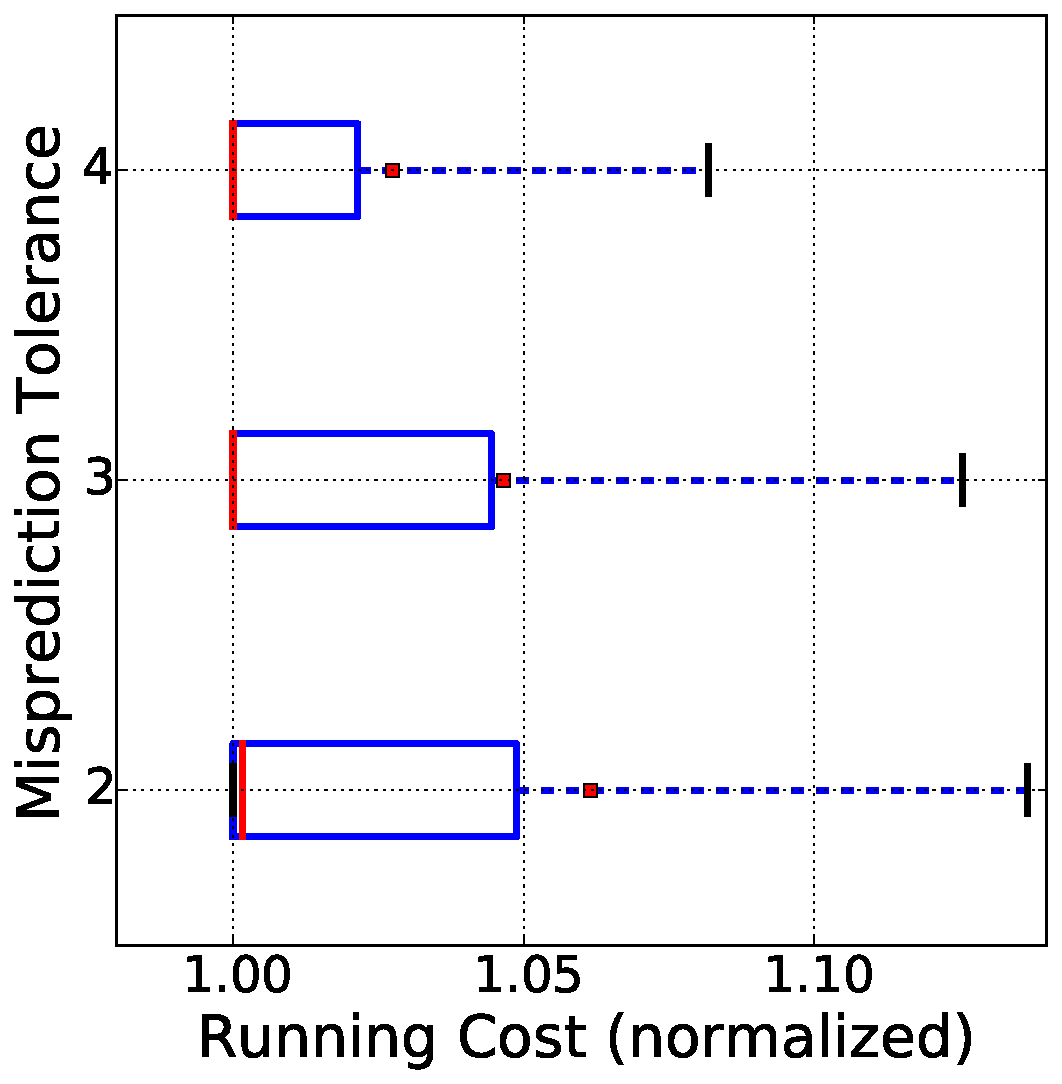
\includegraphics[width=\linewidth]{figures/single_cost_tuning_tolerance_performance.pdf}
    \caption{Search Performance}
    \label{fig:single_cost_tuning_tolerance_performance}
\end{subfigure}
\begin{subfigure}[b]{0.4\textwidth}
    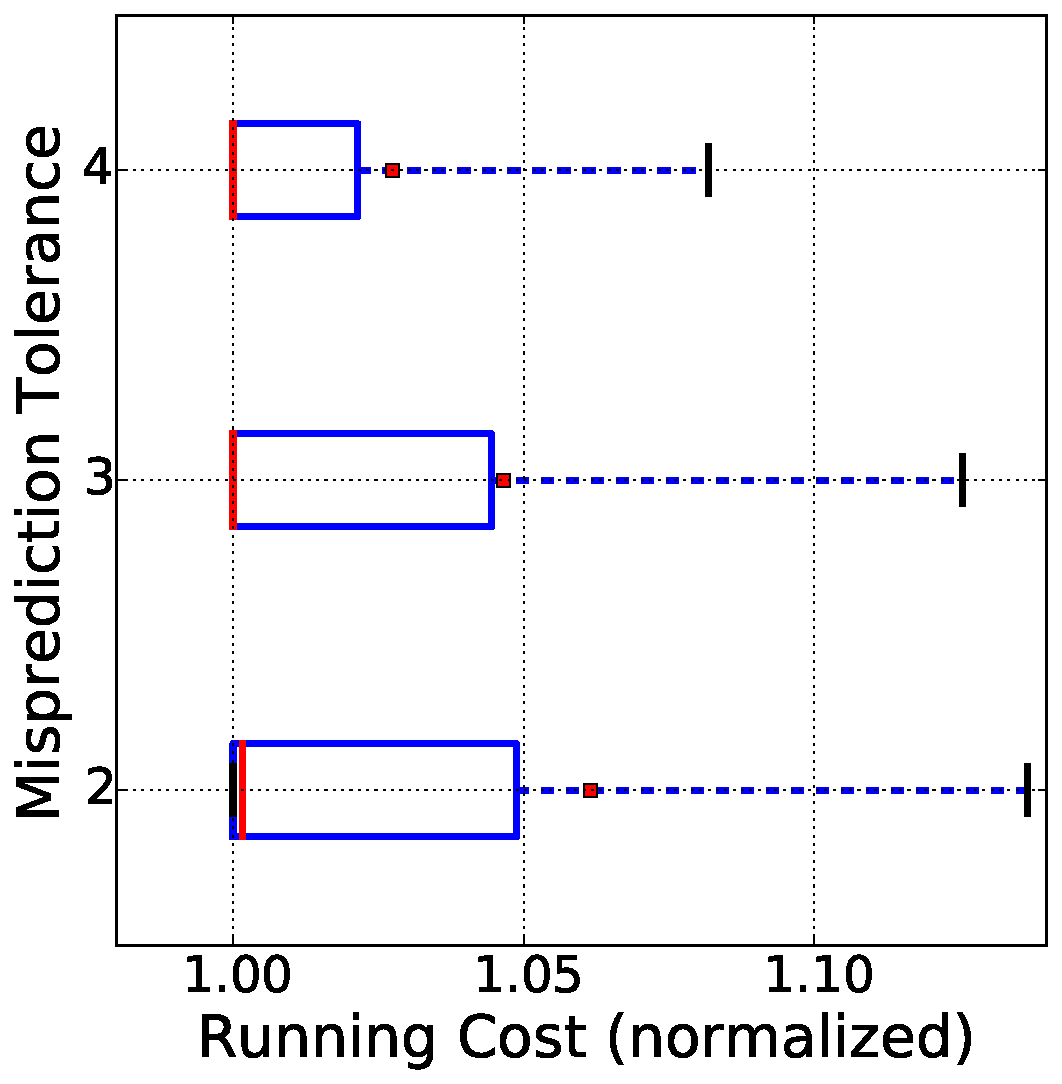
\includegraphics[width=\linewidth]{figures/single_cost_tuning_tolerance_performance.pdf}
    \caption{Search Cost}
    \label{fig:single_cost_tuning_tolerance_performance}
\end{subfigure}
\caption{\small{\textbf{Tuning the misprediction tolerance.} A higher tolerance to mispredictions generates higher search cost.}}
\label{fig:single_misprediction_tolerance}
\end{figure}


\subsection*{Alternative search strategies}
\scout generates the probability vector $P_{i}$
for each new observation (running the workload on $S_i$).
Our current search strategy only uses information from the latest observation.
\scout stores historical observations and therefore,
the next search step can be determined using several past observations.
%In \myfigure{\ref{fig:search_strategies}}, we illustrate a way to incorporate other observations.
Given two observations on $S_1$ and $S_2$ and two unevaluated configuration $S_3$ and $S_4$,
\scout generates prediction probability
$P_{13}$ and $P_{14}$ from $S_1$, and $P_{23}$ and $P_{24}$ from $S_2$.
Instead of choosing $P_{23}$ after the second step,
\scout should choose $P_{14}$ when $S_2$ is much worse than $S_1$ (due to mispredictions).
This strategy is more likely to avoid bad choices.
On the other hand, 
\scout currently relies on offline performance modeling.
Another alternative is to update the prediction model upon new observations.
For unseen workloads, this update enables \scout to improve prediction accuracy.
However, the downside is the cost of retraining the model.
An online learning method might help reduce the retraining cost.
The two possible alternatives remain as future work.

\begin{figure}[!htbp]
 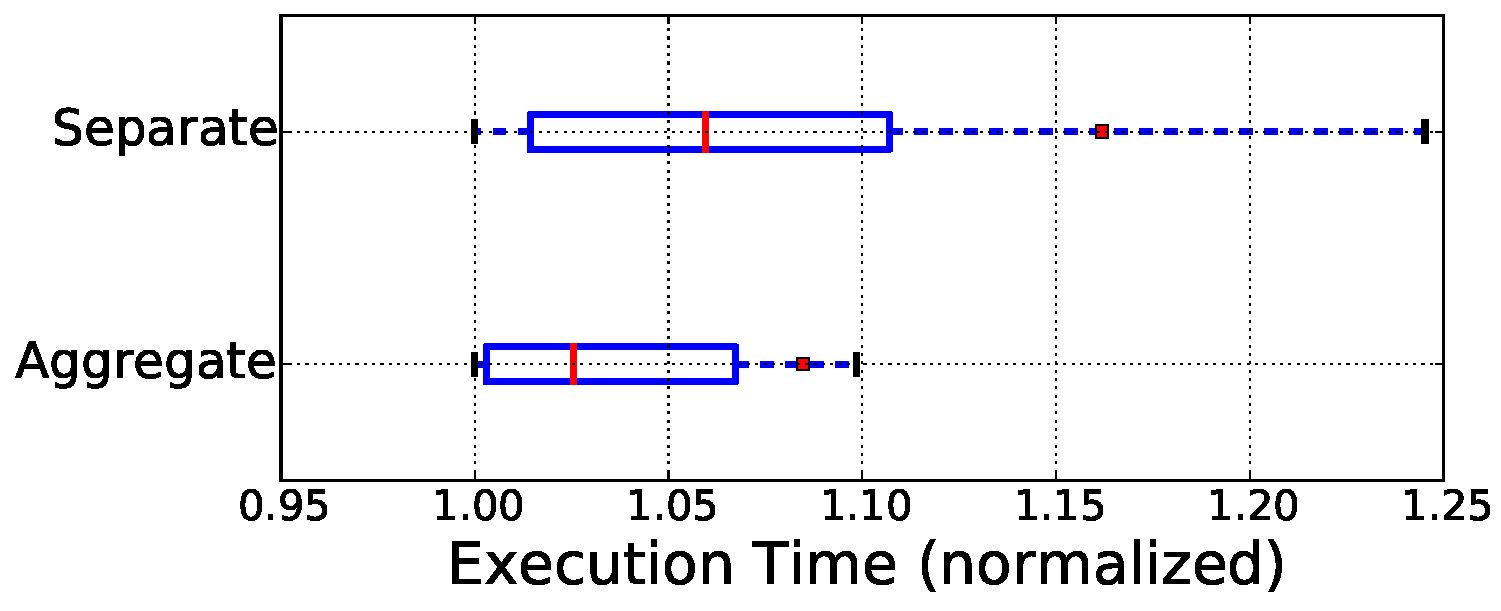
\includegraphics[width=.8\textwidth]{figures/multiple_size_of_dataset.pdf}
 \centering
 \caption{\textbf{Universal performance models.}
 Training data form multiple systems improves prediction.}
 \label{fig:prediction_accuracy_comparison}
\end{figure}

\textbf{Universal Prediction Models.}
% The performance models are built to find the best cloud configuration for a certain workload. These performance models generalize the information learned from the evaluated configurations. This helps the model to be accurate while predicting new cloud configurations. 
In prior work, the performance model needs to be retrained
for every optimization process, which leads to wasted effort.
There is a need for a modeling strategy, which becomes more accurate with experience. 
% This experienced model is useful in our setting, since measuring a new cloud configuration can be resource intensive. 
Transfer learning can be beneficial in our setting,
where the performance model can predict a new workload
using knowledge learned from optimization results of other workloads~\cite{pan2010survey}.
\scout tries to learn from other performance data so that all the experience from the past optimization process is not lost.
Figure~\ref{fig:prediction_accuracy_comparison} shows
how the performance model learned from more data (from different workloads) can
generalize better than the performance model training for a single application.
In the figure, the horizontal axis represents the execution time of the workload,
and the vertical axis shows two versions of \scout. \emph{Separate}
refers to the \scout which is trained with performance data from just
Hadoop workloads, whereas \emph{Aggregate} refers to \scout trained on Hadoop
as well as Spark workloads. We can see that \emph{Aggregate} can find cloud
configurations with better performance (lower execution time). 
\textit{Overall, the prediction model used in \scout is universal and can learn from any workload.}

\subsection*{Time-cost trade-off}
Often a
user is willing to wait longer for a result if there is a big
reduction in cost.
For example, many might be willing to trade a 20\% increase execution time for a 50\% decrease in running cost.
This is similar to the energy-time trade-off in high-performance computing~\cite{Freeh2007}.
\scout can support this scenario.
In our design, we define prediction classes based on the normalized performance of a single performance measure, \ie{time or cost}.
Previous work supports this trade-off in a similar manner~\cite{Hsu2018Arrow}.
%We instead define the classes based on the normalized performance of the product of time and cost.
%In our previous work, we show that how to support time-cost trade-off in a search-based method~\cite{Hsu2018Arrow}.
%We plan to support this feature in \scout.


\section{Conclusion}
\label{sec:conclusion}

Cloud architecture tuning (CAT) is essential
to maximize the performance of an application
while keeping the deployment cost down.
In this chapter, we identify key elements for an effective CAT method.
We design and implement a novel system \scout, which delivers
\emph{efficient}, \emph{effective} and \emph{reliable} search performance.


%Today most applications are hosted in the cloud.
%It is essential to maximize the performance of an application while keeping the deployment cost down.
%Machine learning and sampling techniques have been previously proposed to
%build models to predict the performance of cloud configurations.
%However, the techniques proposed in prior work are either expensive to train or are unreliable---if trained on %sparse samples. 

%Our method, \scout, is different to the previously proposed directions and promotes learning from previous %experience---optimization process.
%We advocate using historical data to identify regions on the configuration space, which might contain the best cloud configuration. To use the historical data, we propose a new modeling scheme which use low-level metrics along with pair-wise modeling technique to transfer knowledge from one optimization process to the other.

